\documentclass{beamer}

\usepackage{graphicx}
\graphicspath{{images/}}

\usecolortheme{seahorse}
\usepackage[latin1]{inputenc}

%\usepackage{bookman}
\usetheme{Madrid}

\newcommand{\bi}{\begin{itemize}}
\newcommand{\ei}{\end{itemize}}

%--------------------------------------

\title{Time series}
\author{Francisco F\"orster Bur\'on}
\date{\today}
\institute[Univ. de Chile]{AS4501}

\begin{document}

\frame{\titlepage}

\section[Outline]{}
\frame{\tableofcontents}


%%%%%%%%%%%%%%%%%%%%
\section{Bibliography}

\frame{
  \frametitle{Bibliography}
  \bi
    \item Modern Statistical Methods for Astronomy, with R Applications. E. Feigelson, G. Babu.
    \item Statistics, Data Mining, and Machine Learning in Astronomy, A Practical Python Guide for the Analysis of Survey Data. Z. Ivezic, A. Connolly, J. VanderPlas, A. Gray
  \ei
}


%%%%%%%%%%%%%%%%%%%%
\section{Variable phenomena}

\frame{
  \frametitle{Variable phenomena}
  \bi
    \item Apparent: rotation, orbital motions
      
      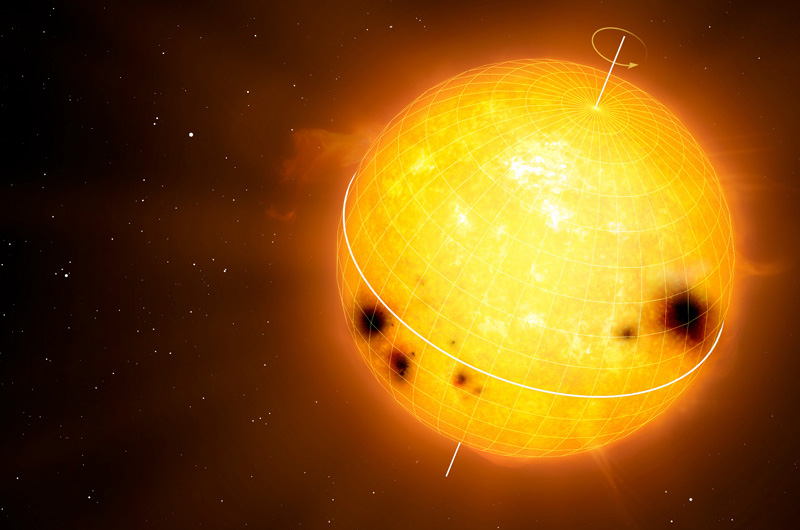
\includegraphics[scale=0.16]{spots.jpg}

    \item Intrinsic: pulsations, explosions, ejections, accretion

        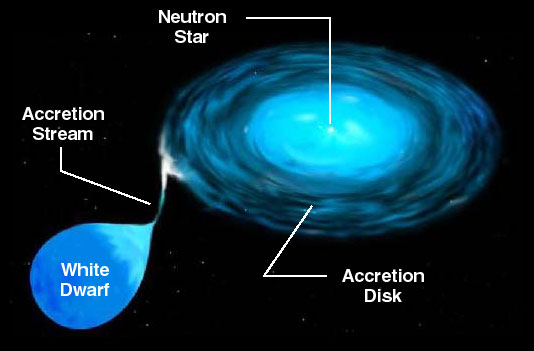
\includegraphics[scale=0.3]{accretion.jpg}

  \ei
}

\frame{
  \frametitle{Variable phenomena}
      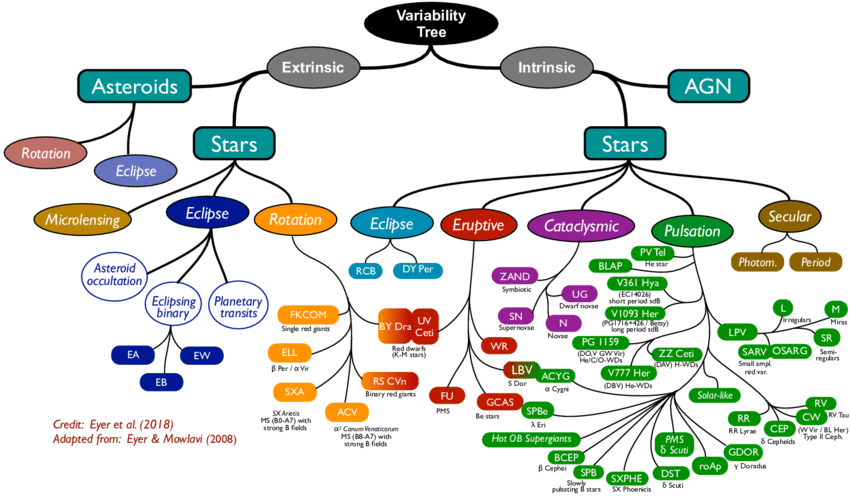
\includegraphics[scale=0.4]{eyer.png}
      \footnotesize{See \url{https://www.youtube.com/watch?v=Pcy4U5uvL8I}}
}

%\frame{
%  \frametitle{Variable phenomena}
%  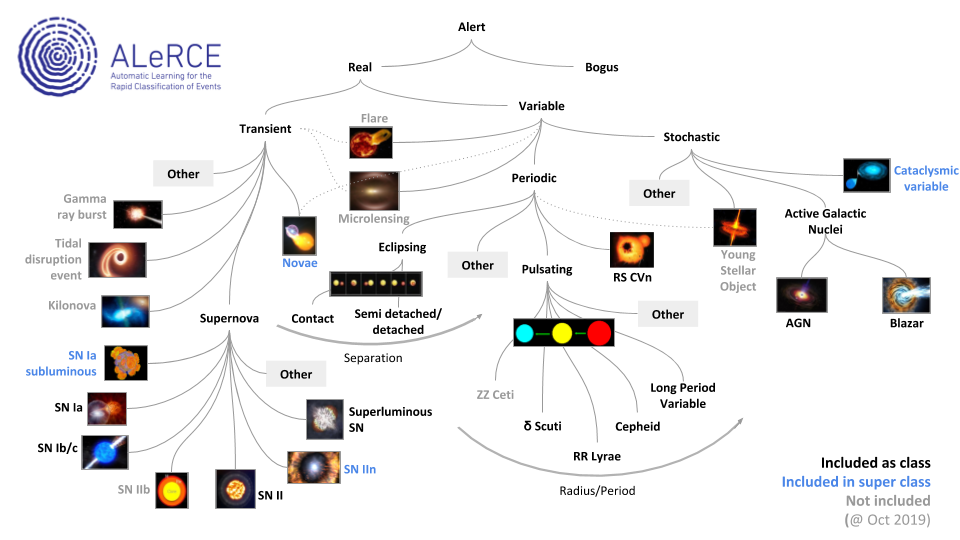
\includegraphics[scale=0.35]{taxonomy.png}
%  
%}

%%%%%%%%%%%%%%%%%%%%
\section{Timescales in astronomy}

\frame{
  \frametitle{Timescales}
  \bi
    \item Binary star orbits: minutes to centuries
    \item Rotation: msec to months

        \vspace{.5cm}
        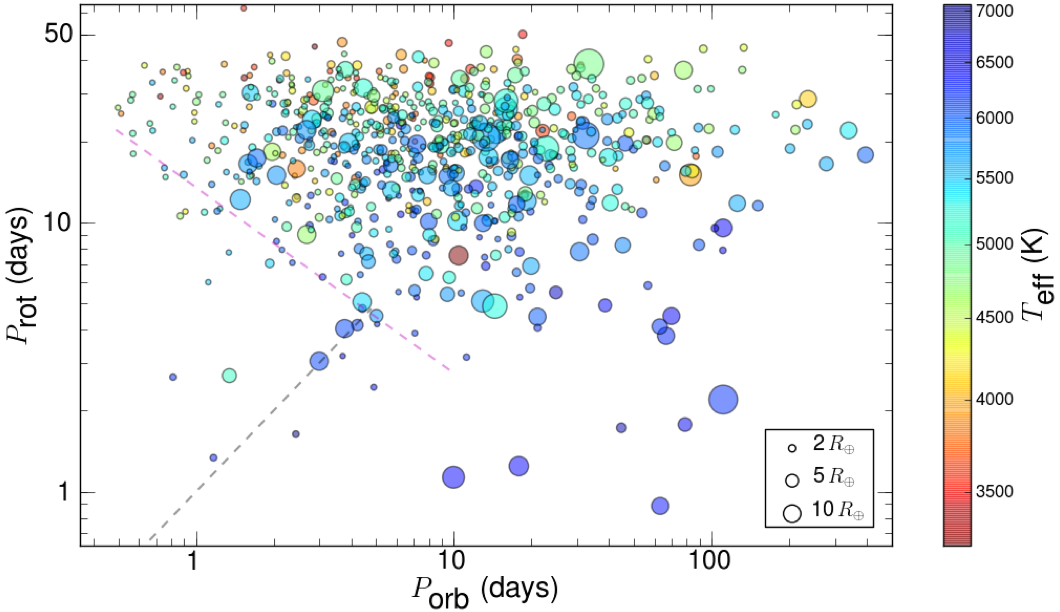
\includegraphics[scale=0.2]{rotation.png}

    \item Accretion: $\mu$sec to decades
    \item Explosions: seconds to years
  \ei
}

%%%%%%%%%%%%%%%%%%%%
\section{Surveys}

\frame{
  \frametitle{Astronomical surveys}

  \bi
  \item Main variable: \emph{etendue} = area x field of view

\vspace{.5cm}
        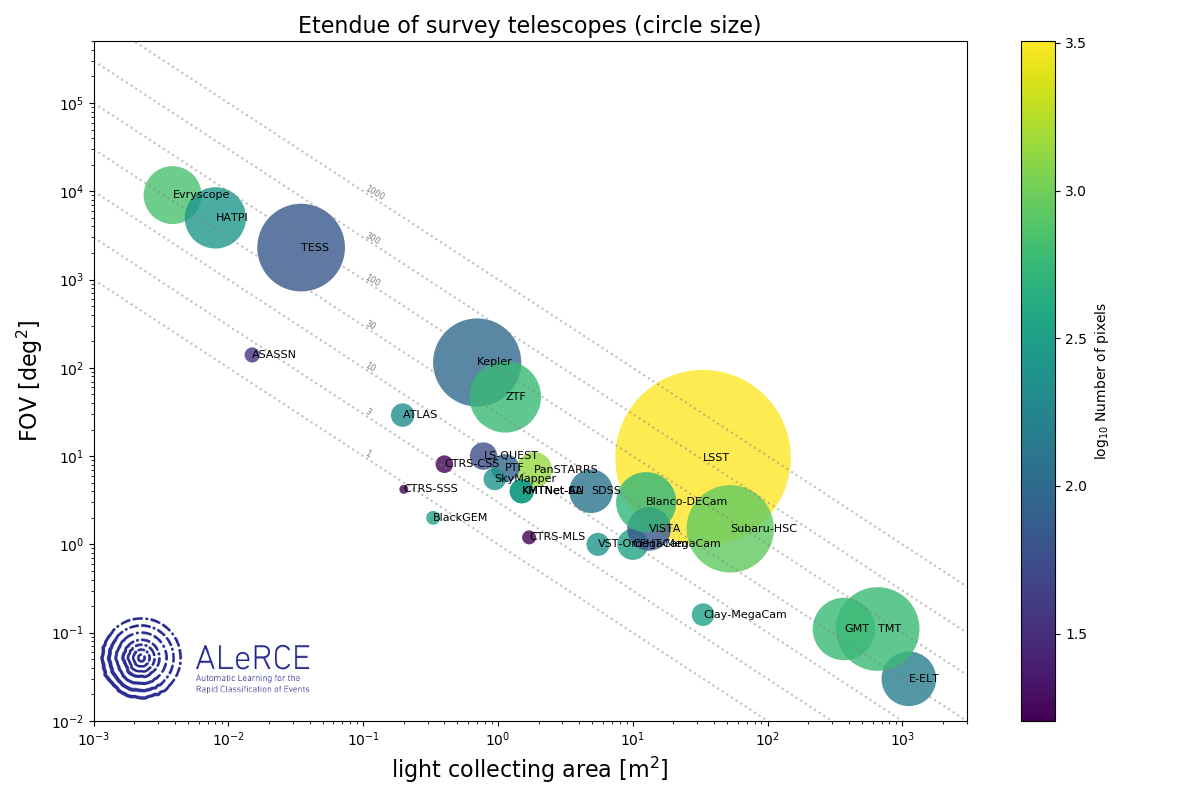
\includegraphics[scale=0.35]{etendue.png}
%{\tiny
%
%\begin{tabular}{l c c c c} 
%
%  Camera & Light--collecting area  &  Field of view  & Etendue & Number of pixels \\ 
%
%  & [m$^2$] & [deg$^2$] & [m$^2$ deg$^2$]  & [Mpix] \\
%
%\hline
%
%      OmegaCam & 5.3 & 1 &  5.3 & 268 \\%& Paranal \\
%
%  iPTF & 1.1 & 7.8 & 8.6 & 92 \\%& Palomar \\
%
%  SkyMapper & 1.4 & 5.7 & 8.2 & 256 \\%& SSO \\ 
%
%  PS1  & 2.5 & 3 & 7.6 & 1400 \\%& Haleakala \\
%
%  Dark Energy Camera (DECam) & 11.3 & 3 & {\bf 33.9} & 520 \\%& CTIO \\
%
%  Hyper Suprime Camera (HSC) & 52.8 & 1.5 & {\bf 79.2} & 870 \\%& Mauna Kea \\
%
%  \hline 
%
%  KMTNET (x3) & 2.0 & 4 & 8. & 340 \\%& CTIO, SAAO, SSO \\
%
%  ZTF & 1.1 & 47 & 51.7 & 576 \\%& Palomar \\
%
%  LSST  Comm. Cam. & 35.7 & 0.4 & 14.5 & 144 \\%& CTIO \\
%
%  LSST & 35.7 & 9.6 & {\bf 344.2} & 3200 \\%& CTIO \\
%
%\end{tabular}
%}
    \ei
}

\frame{
        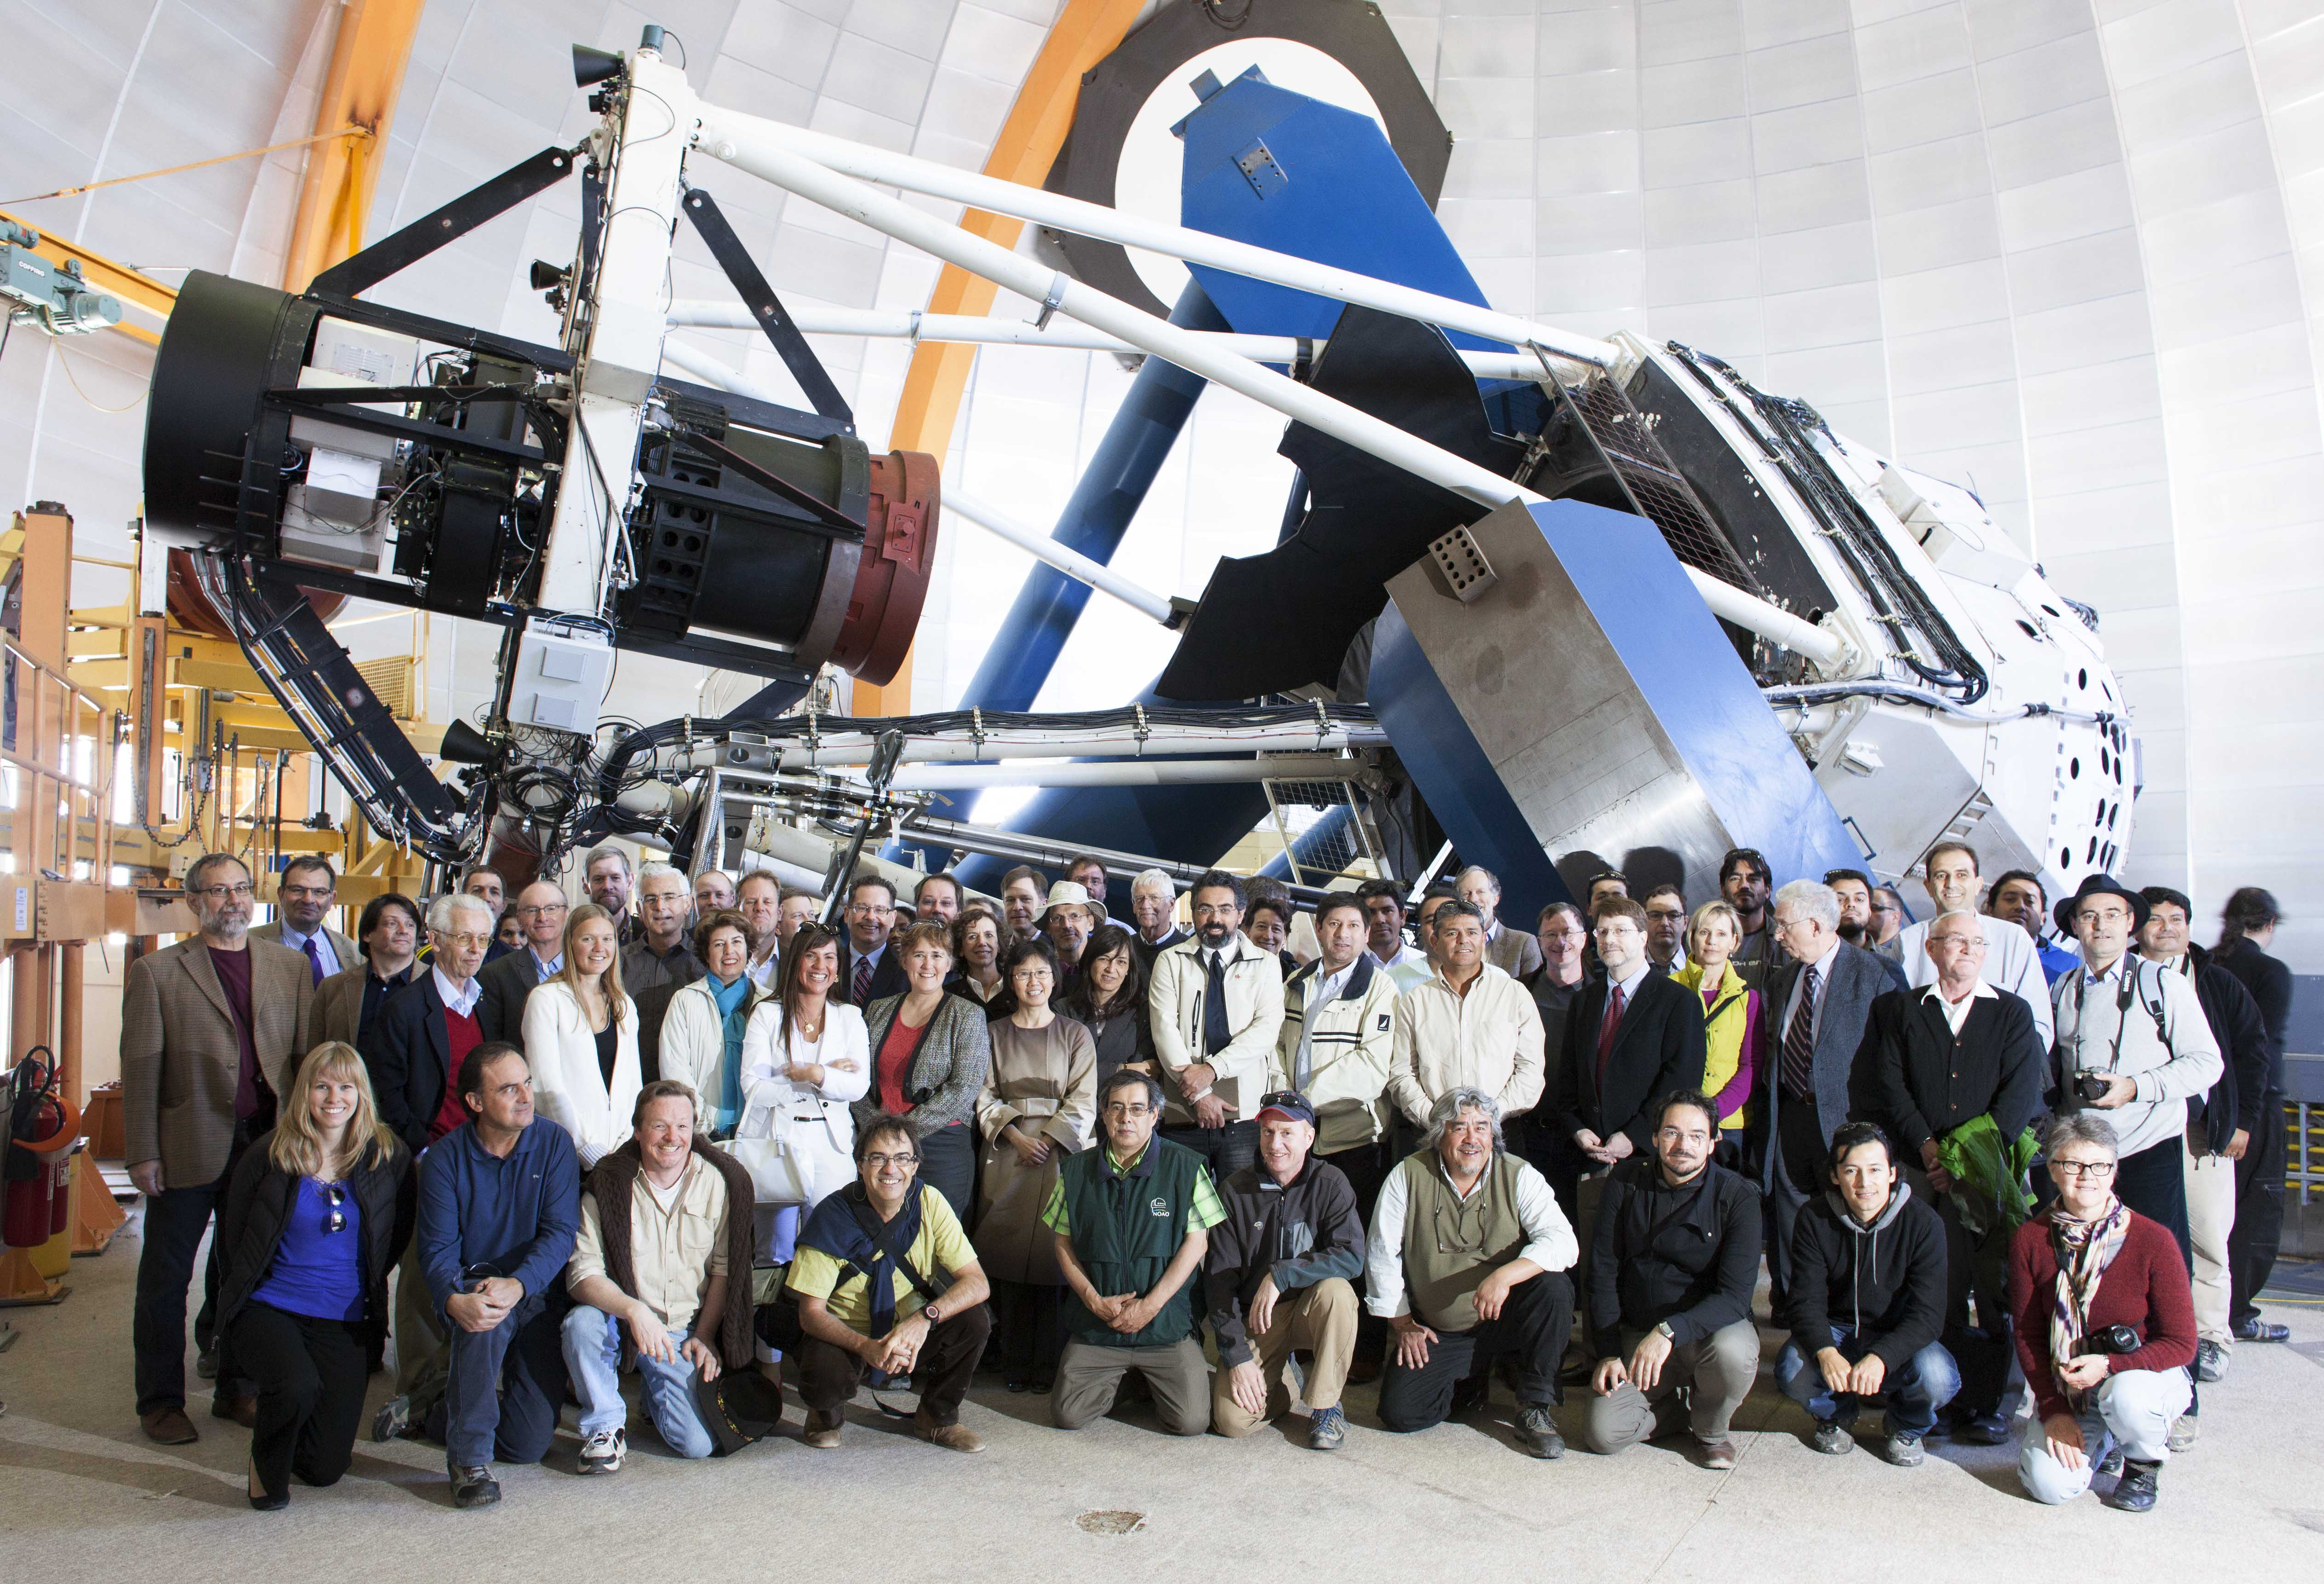
\includegraphics[scale=0.2]{DECam.jpeg}

        The Dark Energy Camera on the Blanco telescope.
}  

\frame{
        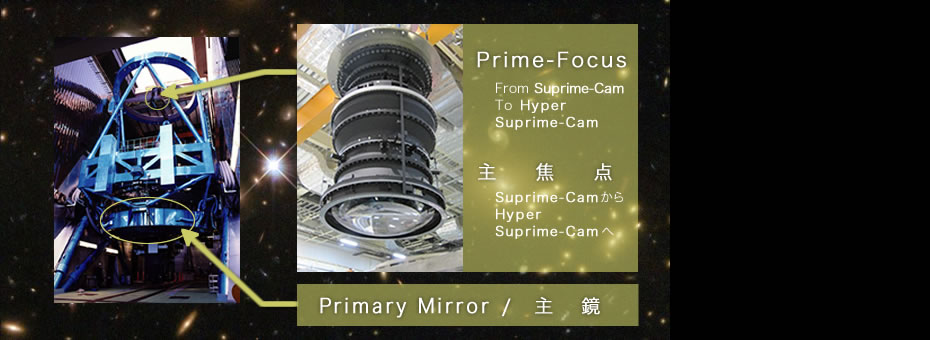
\includegraphics[scale=0.5]{HSC.jpg}

        The Hyper Suprime Camera on the Subaru Telescope.
}  

\frame{
        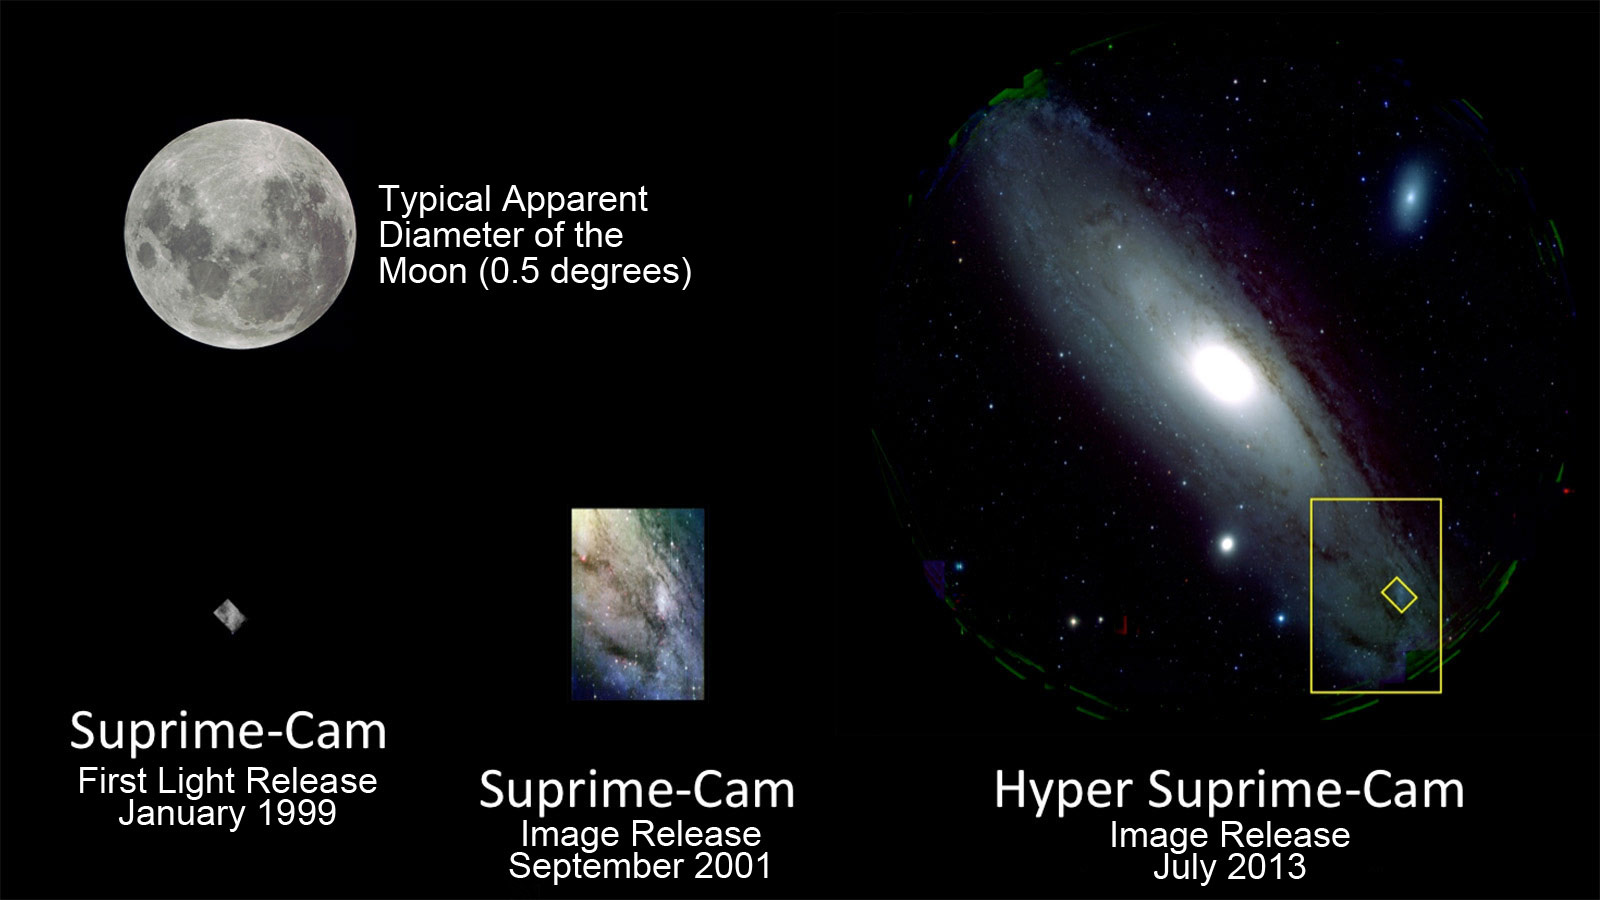
\includegraphics[scale=0.2]{HSC_FoV.jpg}
}  

\frame{
        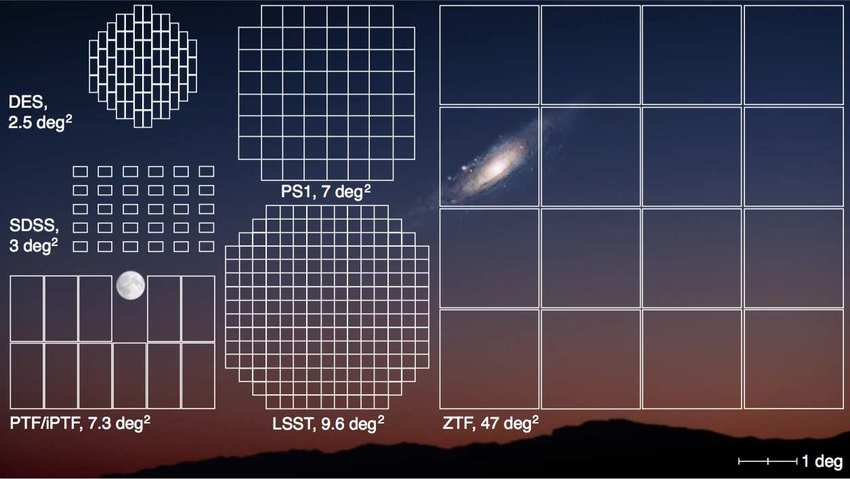
\includegraphics[scale=0.4]{ZTF.png}

}  

\frame{
        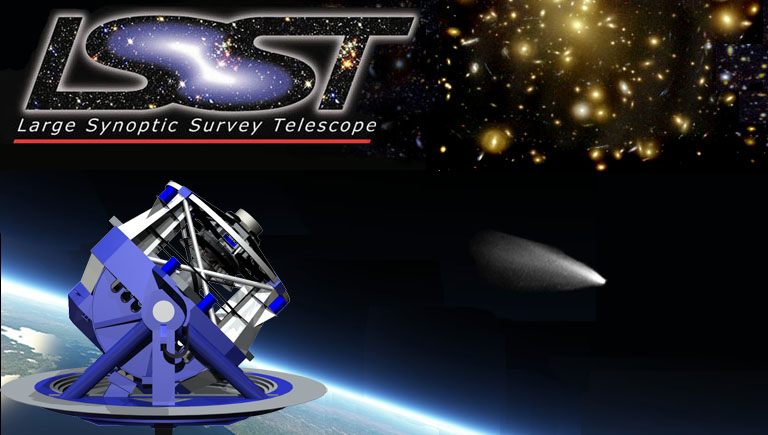
\includegraphics[scale=0.5]{lsst.jpg}

        The future Large Synoptic Survey Telescope (LSST).
}  

\frame{
        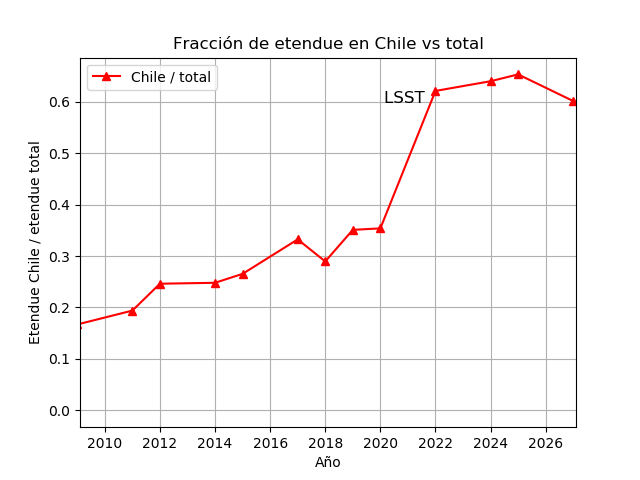
\includegraphics[scale=0.75]{etenduefrac.png}

}  

\frame{
  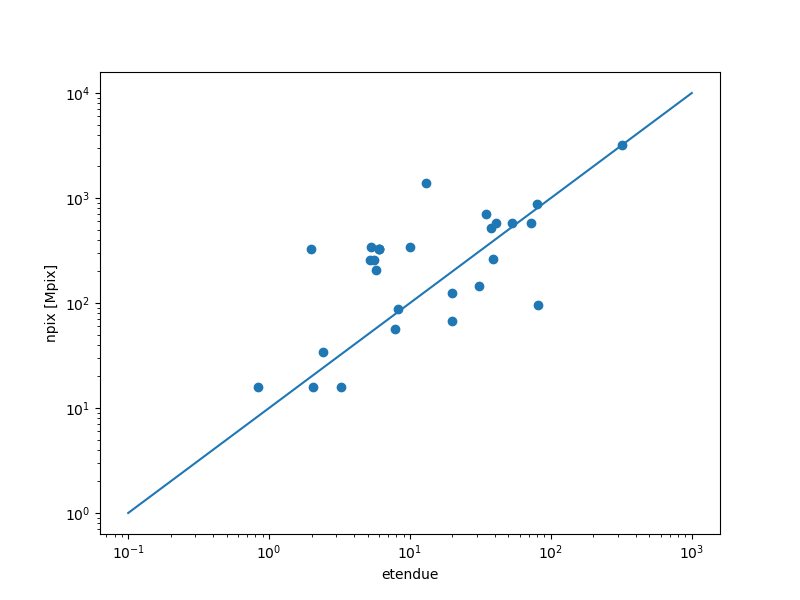
\includegraphics[scale=0.6]{etenduenpix.png}

  Large etendue $\approx$ big data

}  

\frame{


  \begin{center}
    {\huge I. Stochastic autoregressive models}
  \end{center}

}


\section{Stochastic process}

\frame{
  \frametitle{Stochastic processes}
  
  In probability theory, a {\bf stochastic process}, or sometimes random process, is a collection of random variables representing the evolution of some system of random values over time. This is the probabilistic counterpart to a deterministic process (or deterministic system).
}

%%%%%%%%%%%%%%%%%%%%
\section{Statistical behaviour in astronomy}

\frame{
  \frametitle{Statistical behaviour - 1/$f^{\gamma}$ noise}
  
  \bi
\item Power spectral density $S(\nu) \propto 1/{f^{\gamma}}$ 

%  \only<1>{
%    $x(t) = \sum_k A_k sin(2 \pi \nu_k t + \phi_k), ~~~S(\nu) = \sum_{k: \nu_k < \nu} A_{k}^2 / 2$
%  }

\item white (Gaussian, no correlation in time, f = 0), pink (long
  memory, f = 1), red or brown (random walk, f = 2)

        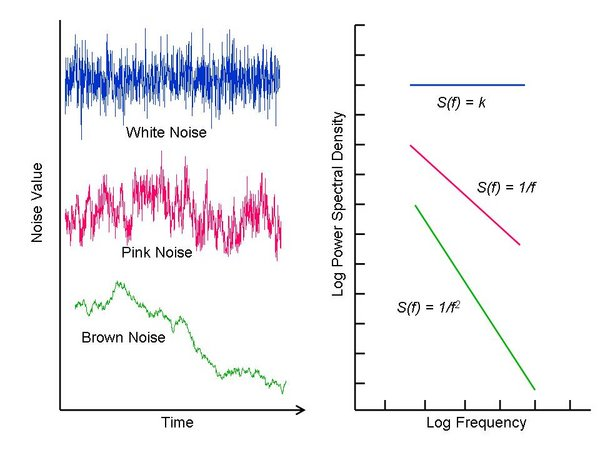
\includegraphics[scale=0.45]{types_of_noise.jpg}

\item Existence of 1/f noise is one of the oldest puzzles of physics

  \ei
}

\frame{
  \frametitle{Statistical behaviour -- Explosive}

  Diversity of behaviours depend on physical mechanism
  
  \bi

\item Magnetic reconnection
\item Scintillation
\item Relativistic  jets
\item Microlensing
\item Supernova
\item Thermonuclear explosions
\item Black hole birth
\ei
 }



%%%%%%%%%%%%%%%%%%%%
\section{Astronomical data}

\frame {
	\frametitle{Astronomical Data}
	\bi
      \only<1>{
		  \item Irregular sampling / Gaps

        \vspace{.5cm}
        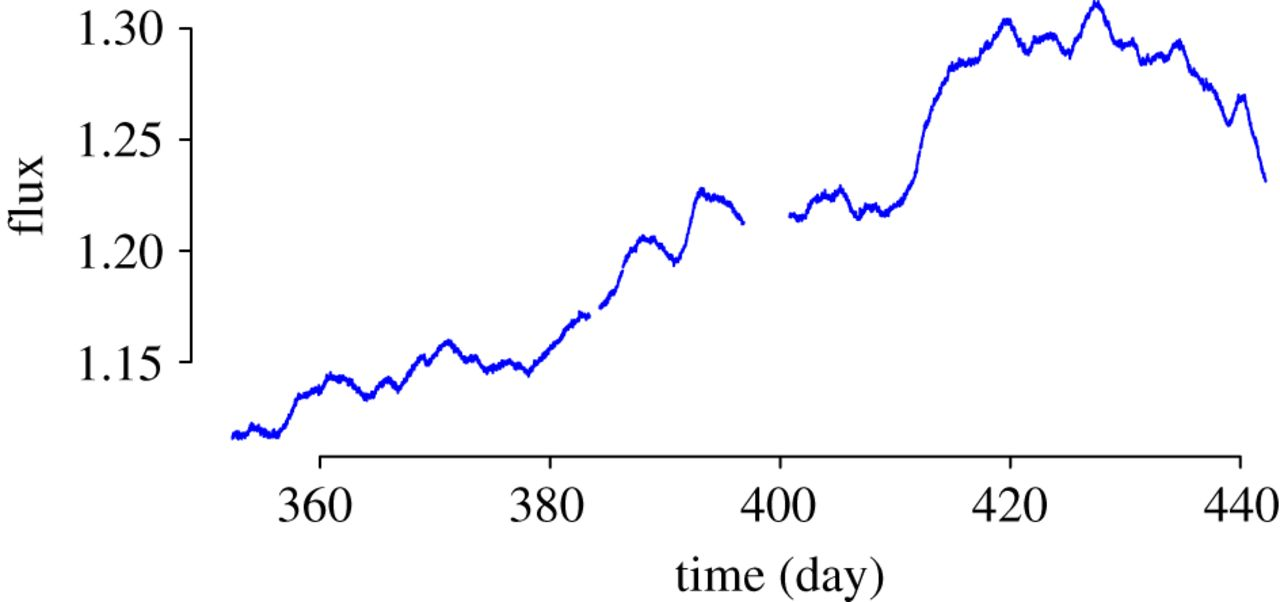
\includegraphics[scale=0.7]{uneven.jpg}
      }
        
      \only<2>{
		  \item Heteroscedastic errors
        
        \vspace{.5cm}
        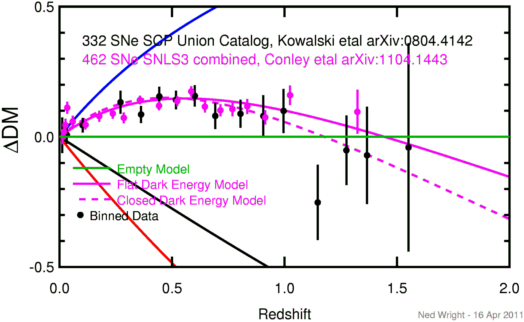
\includegraphics[scale=0.4]{heteroskedasticity.png}
      }

      \only<3>{
		  \item Low signal to noise ratio

        \vspace{.5cm}
        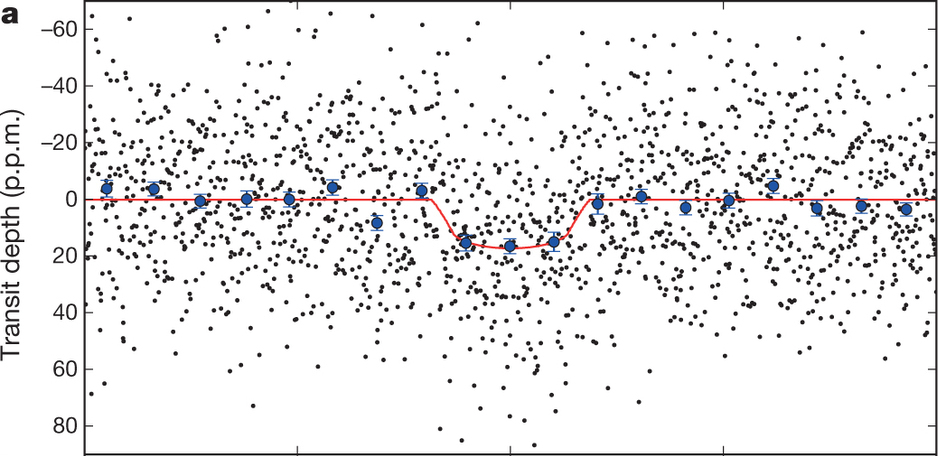
\includegraphics[scale=0.2]{lowSNR.jpg}
      }
	\ei
}

\frame{
  \centering
  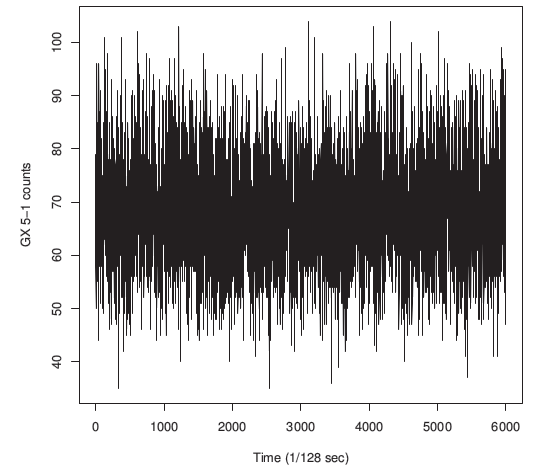
\includegraphics[scale=.4]{timeseries.png}

  Time series of the X--ray emission from the galactic X--ray binary system GX 5--1 measured from the Ginga satellite observatory.
    
}



%%%%%%%%%%%%%%%%%%%%
\section{Variability modeling}


\frame{
  \frametitle{Variability modeling}

  \bi
  \item Deterministic trends: Regression analysis
  \item {\bf Stochastic and autocorrelated: Autoregressive models}
  \item Periodic signal: Fourier transform and related Harmonics analysis
    \ei

    \vspace{2cm} Procedures for all the above are well developed for
    evenly spaced data. Theory for uneven sampling and heteroscedastic
    errors is still being developed.  }
    

%%%%%%%%%%%%%%%%%%%%
\section{Autocorrelation}

\frame{
  \frametitle{Autocorrelation}
  
  \bi
  \item  Autocorrelation measures correlated structure
  \item $ACF(k) = \frac{\sum_{t = 1}^{n - k}  (x_t - \bar x) (x_{t + k} - \bar x)}{\sum_{t = 1}^{n} (x_t - \bar x)^2}$, ~~~~where k is the lag time
    \item a plot of the autocorrelation function is called a {\bf correlogram}

\vspace{1cm}
\item White noise: $ACF(k) = \begin{cases} 1, & k = 0 \\ 0, & k \ne 0 \end{cases}$
\item Short term autocorrelation: ACF  large for small k
  \item Long term autocorrelation: ACF large for wide range of k
    \item Periodic signal: periodic ACF
    \ei


}


\frame{
  \frametitle{Autocorrelation and autocovariance}
  
  \bi
  \item Autocovariance
  \begin{align}
    \gamma(k) &= E[(x_t - \bar x) (x_{t + k} - \bar x)]\\
    &= \frac{1}{N-1} \sum_{t = 1}^{n - k} (x_t - \bar x) (x_{t + k} - \bar x) \\
  \end{align}
  \item Autocorrelation
  \begin{align}
    ACF(k) &\equiv \rho(k) = \frac{\gamma(k)}{\gamma(0)} \\
    &= \frac{E[(x_t - \bar x) (x_{t + k} - \bar x)]}{E[(x_t - \bar x) (x_t - \bar x)]} \\
    &= \frac{\sum_{t = 1}^{n - k}  (x_t - \bar x) (x_{t + k} - \bar x)}{\sum_{t = 1}^{n} (x_t - \bar x)^2}
  \end{align}
  \ei

}

\frame{
  \frametitle{Stationarity}

  \bi
  \item Stationarity is the property that temporal behaviour, whether
    stochastic or deterministic, is statistically unchanged by an
    arbitrary shift in time
    \item Weakly stationary processes have unchanged moments (e.g. mean or autocovariance)

\vspace{.5cm}
    \item The variance of the mean of a stationary process changes
      when autocorrelation is present
      
      \vspace{.5cm}
      $\hat {var} (\bar x_n) = \frac{\sigma^2}{n} [ 1 + 2 \sum_{k = 1}^{n - 1} (1 - k / n) ACF(k) ]$
      \vspace{.5cm}

      This means that the comparison of means of different objects or
      the same object at different times must take into account the
      increase in variance due to the autocorrelation.

  \ei 

}

\frame{
  \centering
  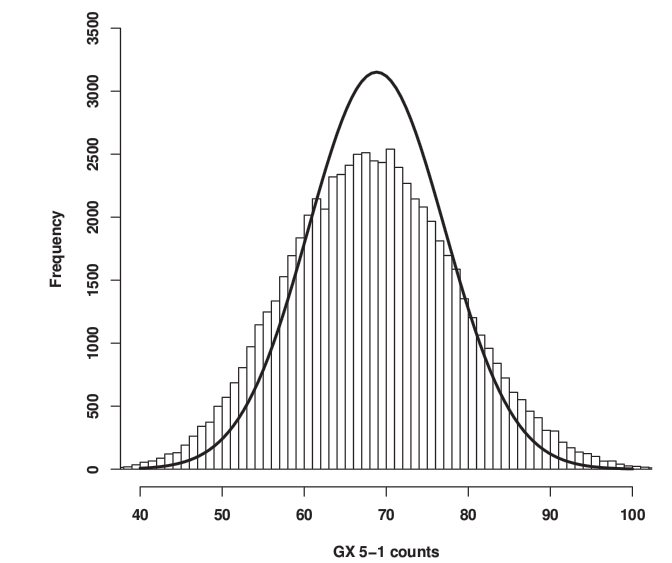
\includegraphics[scale=.35]{histogram.png}

  Histogram of the timeseries of GX 5--1 compared to the best fit
  Gaussian distribution. Excess variance with respect to a white noise
  model is found. Some asymmetry is also observed.
    
}

\frame{
  \frametitle{Smoothing}
  
  \bi
  
  \item Useful for visual exploration of a time series
    
  \item Central moving average (CMA) with bandwidth of j time intervals:
    \begin{align}
      \hat X _{i, CMA}(j) = \frac{1}{j + 1} \sum_{k = -j /2}^{j / 2} X_{i + k}
    \end{align}

  \item Exponentially weighted moving average (EWMA)
    \begin{align}
      \hat X_{i, EWMA} = \alpha X_i + (1 - \alpha) X_{i - 1},
    \end{align}
    where $0 \le \alpha \le 1$ 
    \ei
}
    

\frame{
  \centering

  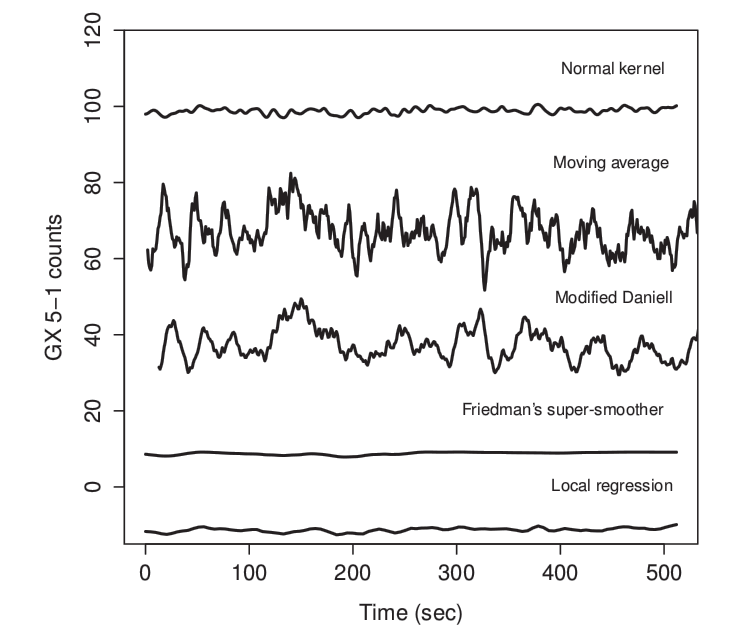
\includegraphics[scale=0.3]{smoothing.png}

  Smoothed timeseries of GX 5--1, showing no obvious non--stationary
  behaviour. However, the source shows stochastic, possibly
  autocorrelated and quasi--periodic, variability. }

\frame{
  \frametitle{Partial autocorrelation function (PACF)}
  
  
  \bi
  \item It gives the autocorrelation at lag time k removing the effects of correlations at shorter lags
  \item It is found by successively fitting autoregressive models with order 1, 2, ... p and setting the last coefficient of each model to the PACF parameter.
    \item PACF is useful to understand the timescales responsible for the autocorrelated behaviour
  \ei 

}

\frame{
  \centering
  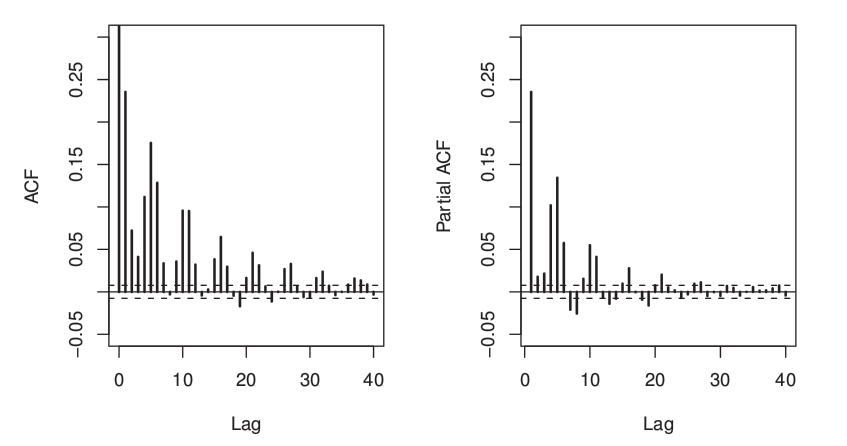
\includegraphics[scale=.4]{ACF.png}

  Autocorrelation function (ACF) and partial autocorrelation function
  (PACF) of the GX 5--1 timeseries. PACF shows that the strongest
  non--zero peak is located between 4--6 increments (autocorrelation),
  but there are weaker peaks at larger lags periodically separated by
  5--6 increments up to 20--30 increments (quasi--periodic) .
    
}


\frame{
  \frametitle{Lag k scatter plot}
  
  
  \bi
  \item Scatter plot of x(t + k) vs x(t)
  \item A useful diagnostic to understand autocorrelation structure
  \item No structure: uncorrelated noise
  \item Linear: Stochastic autoregression
  \item Circular: periodic signal
  \item Clusters: Non--stationarity
  \ei 

  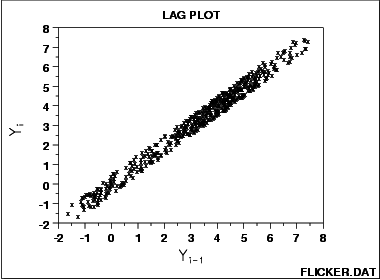
\includegraphics[scale=.4]{lagplot.png}

}

\frame{
  \frametitle{Durbin--Watson statistic}
  

  \bi
  \item Useful statistic that is a simple measure of autocorrelation in an evenly spaced time series:

    \vspace{.4cm}
    $d_{DW} = \frac{\sum_{i = 2}^{n} (x_i - x_{i - 1})^2}{\sum_{i = 1}^{n} x_i^2}$ ~~~~~$\begin{cases} 0 \le d_{DW} < 2, & positive~ autocorrelation \\  d_{DW} = 2, & no~ autocorrelation \\ 2 < d_{DW} \le 4, & negative~autocorrelation \end{cases}$
  \ei 
}

%%%%%%%%%%%%%%%%%%%%
\section{Stochastic autoregressive models}

\frame{
  
  \frametitle{Stochastic autoregressive models}
  
\bi
\item Simplest stochastic autocorrelated model:

\vspace{.3cm}

  $X_i = X_{i - 1} + \epsilon$
\vspace{.3cm}

$\Rightarrow$
\vspace{.3cm}

  $X_i = X_0 + \epsilon_1 + \epsilon_2 + ... + \epsilon_i$~~~  (random walk)

\vspace{.3cm}
\item $ACF_{RW}(i, k) = \frac{1}{1 + k / i}$
\ei
}

\frame{
  \frametitle{Autoregressive (AR) models}

  \bi

  \item $AR(p)$ model:
  \vspace{.3cm}
  \begin{align}
    X_i = \alpha_1 X_{i - 1} + \alpha_2 X_{i - 2} + ... + \alpha_p X_{i - p} + \epsilon_i
  \end{align}
  where $\epsilon_i \sim N(0, \sigma_i^2)$ or white noise

  \vspace{.6cm}

  \item The effect of the error terms is infinite in time.

  \vspace{.3cm}

\item $AR(1)$ model:
  
  \bi
  
  \item Autocorrelation function for lag k is time invariant for $| \alpha_1 | < 1$:
  
    \vspace{.2cm}
    $ACF_{AR(1)}(k) = \alpha_1^k$
    \vspace{.2cm}
    
    \item ACF decays rapidly for $\alpha_1 \sim 0$, but remains high for $\alpha_1 \sim 1$
    \ei
\ei
}

\frame{
  \frametitle{Autoregressive (AR) models}

  \bi

  \item $AR(p)$ model:
  \vspace{.3cm}
  \begin{align}
    X_i = \alpha_1 X_{i - 1} + \alpha_2 X_{i - 2} + ... + \alpha_p X_{i - p} + \epsilon_i
  \end{align}
  where $\epsilon_i \sim N(0, \sigma_i^2)$ or white noise

  \vspace{.6cm}

\item In AR(1), $\alpha_1 = 0$ is equivalent to white noise
\item In AR(1), $\alpha_1 = 1$ is equivalent to a random walk
\vspace{.3cm}
\item For stationary data:
      \bi
      \item In AR(1) we need $-1 < \alpha_1 < 1$
      \item In AR(2) we need $-1 < \alpha_2 < 1, ~~ \alpha_1 + \alpha_2 < 1, ~~ \alpha_2 - \alpha_1 < 1$
      \ei
\ei
}


\frame{
  \centering
  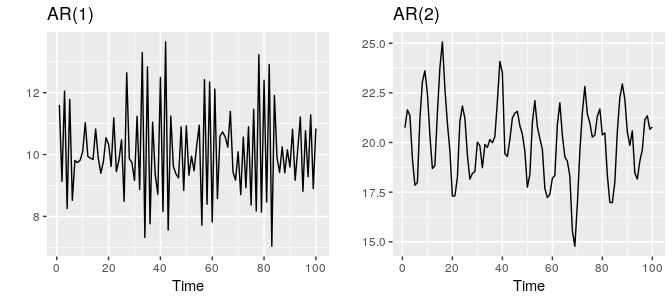
\includegraphics[scale=.6]{AR1AR2.png}

  Example of AR(1) and AR(2) timeseries.
    
}

\frame{
  \centering
  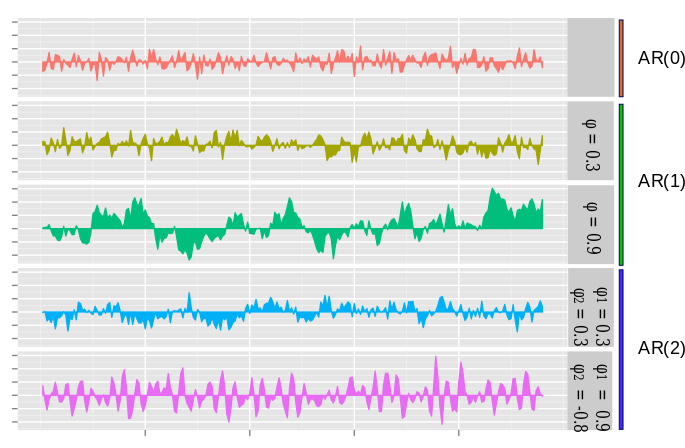
\includegraphics[scale=.4]{ArTimeSeries.png}

 More AR timeseries examples.
    
}

\frame{
  \frametitle{Moving average (MA) models}
  
  \bi
  \item $MA(q)$ model:
  \vspace{.3cm}
  \begin{align}
    X_i = \epsilon_i + \beta_1 \epsilon_{i - 1} + ... + \beta_q \epsilon_{i - q}
  \end{align}
  where $\epsilon_i \sim N(0, \sigma_i^2)$ or white noise.
  \vspace{.3cm}

  \item the current value depends on past values of the noise, but the effect of the error terms is finite in time.

  \item MA models effectively filter high frequency (short timescales)
    noise
    
  \item fitting is more complicated than AR models because the error
    terms are unobserved.

  \ei

}  

\frame{
  \centering
  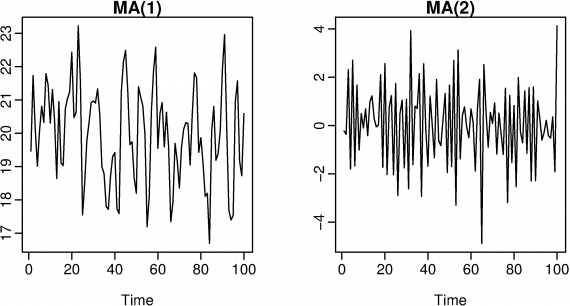
\includegraphics[scale=.4]{MAtimeseries.png}

  Example of MA(1) and MA(2) timeseries
    
}


\frame{
  \frametitle{ARMA(p, q) models}
  
  \bi
  \item $ARMA(p, q)$ model:
  \vspace{.3cm}
  \begin{align}
    X_i = \alpha_1 X_{i - 1} + \alpha_2 X_{i - 2} + ... + \alpha_p X_{i - p}  + \epsilon_i + \beta_1 \epsilon_{i - 1} + ... + \beta_q \epsilon_{i - q}
  \end{align}
  where $\epsilon_i \sim N(0, \sigma_i^2$)
  \vspace{.3cm}

\item ARMA models can be fitted via least square minimization
\item The difficult part is the choice of $p$ and $q$

  \ei

}  


\frame{
  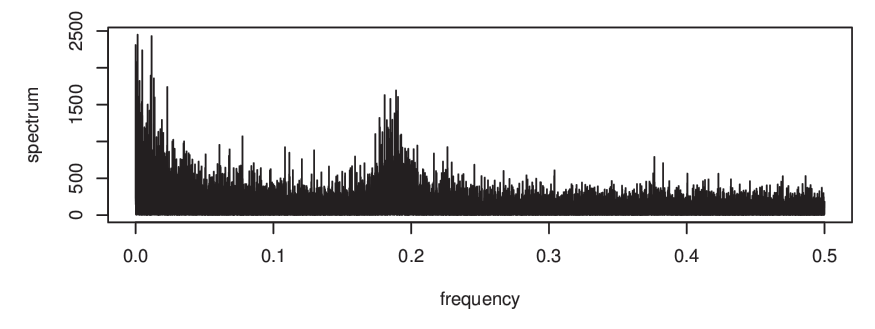
\includegraphics[scale=.4]{spectrum.png}

  Periodogram of the GX 5--1 timeseries.
    
}

\frame{
  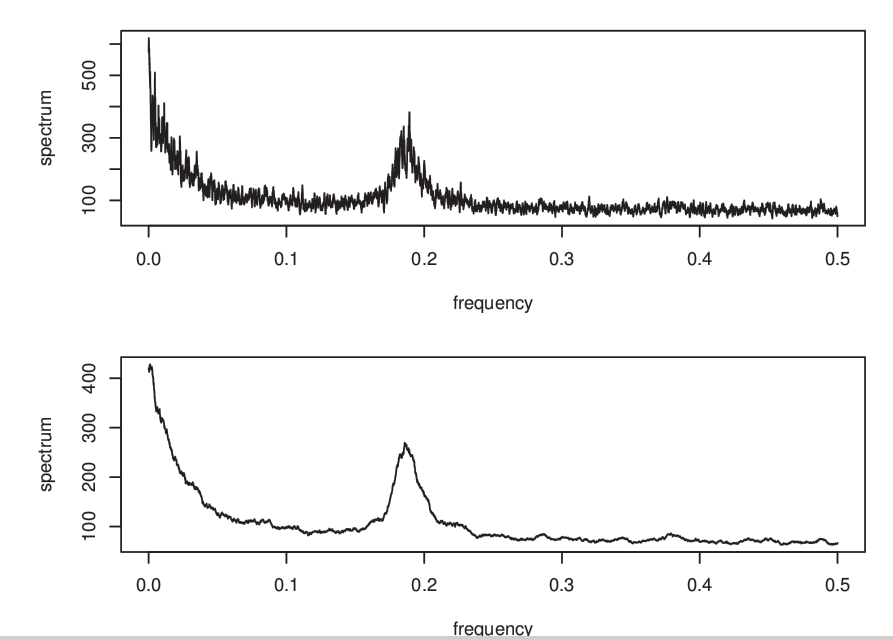
\includegraphics[scale=.35]{spectrum_smoothed.png}

  Smoothed Periodogram of the GX 5--1 timeseries.
    
}

\frame{
  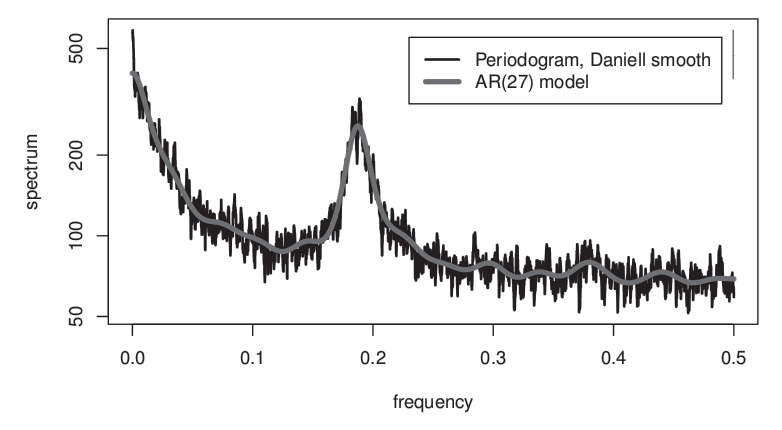
\includegraphics[scale=.4]{AR(27).png}
    
  AR(27) best fit model to the GX 5--1 timeseries.
}

\frame{
  \frametitle{Akaike information criterion (AIC, Akaike 1974)}
  
  \bi
  \item A model selection tool that takes into account the likelihood
    of the model under consideration and the number of parameters used
    in the model.
  \item For a model with $p$ parameters $\theta_p$:
    \begin{align}
      AIC(\theta_p) = -2 \ln(L(\theta_p)) + 2 p
    \end{align}
    where $L(\theta_p)$ is the likelihood of the model under
    consideration
    
    \item The model with the lowest AIC should be used.

      \item For AR(p) models, the AIC reduces to:
        \begin{align}
          AIC(p) = N \ln(\hat \sigma^2) + 2 p
        \end{align}
        where $\hat \sigma_p^2$ is the maximum likelihood estimator (likelihood of the data given the model) of the variance of the $\epsilon$ noise terms.

  \ei }
  
\frame{
  \centering
  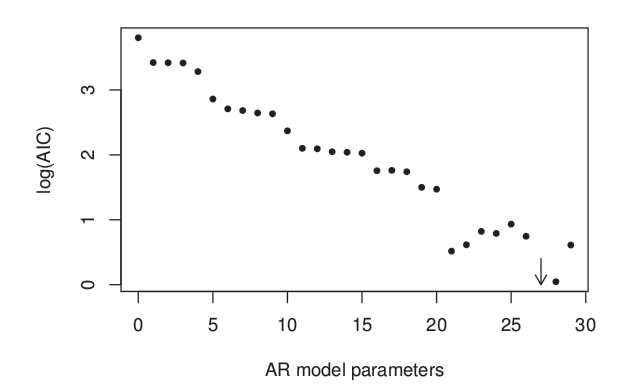
\includegraphics[scale=.4]{AIC.png}
    
  Akaike information criterion for the AR(p) model on the GX 5--1
  timeseries. Best fit model was AR(27) based on this criterion.
}

\frame{
  \frametitle{Bayesian information criterion (BIC, Schwarz 1978)}
  
  \bi
  \item BIC penalizes model complexity more heavily. AIC and BIC rely on different assumptions.
  \item For a model with $p$ parameters $\theta_p$:
    \begin{align}
      BIC(\theta_p) = -2 \ln(L(\theta_p)) +  \ln(n) p
    \end{align}
    where $L(\theta_p)$ is the likelihood of the model under
    consideration and $n$ is the sample size.
    
    \item The model with the lowest BIC should be used.

      \item For AR(p) models, the BIC reduces to:
        \begin{align}
          BIC(p) = N \ln(\hat \sigma^2) + \ln(n) p
        \end{align}
        where $\hat \sigma_p^2$ is the maximum likelihood estimator (likelihood of the data given the model) of the variance of the $\epsilon$ noise terms.

  \ei }

\frame{
  \frametitle{Other models}

  \bi
  \item ARIMA: autoregresive integrated moving average models (Box \& Jenkins 1970)

    Can treat non--stationary stochastic processes

  \item ARCH: autoregressive coditional heteroscedastic 

    Useful for datasets where the variance rather than the local mean changes during the observations

  \item GARCH: generalized ARCH models

    Non--linear dependency on past noise levels

    \ei
  }
  
\frame{
  \frametitle{Irregular Sampling}

  \bi
  \item CARMA: continuous--time autoregressive moving average (Kelly, Becker et al. 2014)
    
    Accounts for irregular sampling and measurement errors. Scales
    linearly with the number of data points, i.e.  for massive
    data sets.

  \item IAR: Irregular Autoregressive model (Eyheramendy et al. 2018)

    \begin{align}
      y_{t_j} = \phi^{t_j - t_{j-1}} y_{t_{j-1}} + \sigma \sqrt{1 - \phi^{2(t_j - t_{j-1})}} \epsilon_{t_j}
    \end{align}
    
    \ei
  }




\frame{
  \frametitle{Application to astronomy}

  \bi

  \item   A timeseries can be represented as

  \begin{align}
    z_t = g(t, \theta) + \delta_t
  \end{align}
  
  where $z_t$ are the observations, $g(t, \theta)$ is a model, and $\delta_t$ are the errors.

\item It is common to assume that $\delta_t$ are independent and Gaussian distributed, but this is not always the case.

\item The solution is to model $z_t - g(t, \theta)$ as an autoregressive model.

  \item To account for irregular sampling one can use CARMA or IAR
  \ei
  }


\frame{

  {\centering

  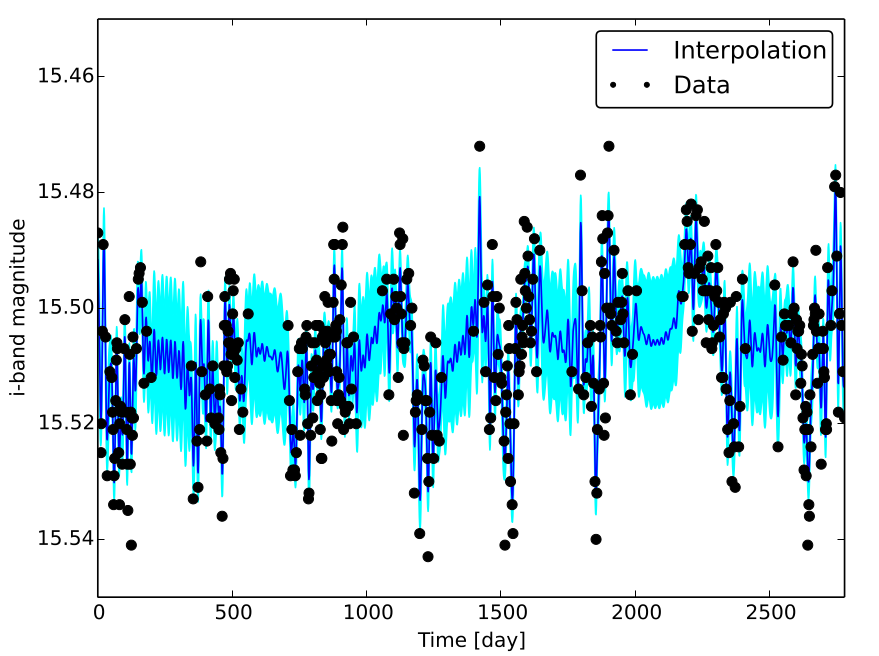
\includegraphics[scale=.3]{CARMA.png}
    
  The i-band light curve for a long-period variable star on the red giant
  branch, from the OGLE-III survey. Also shown is the interpolated light curve
  and its uncertainty assuming a CARMA(6,0) model (Kelly et al. 2014, ApJ).}
}

\frame{

  {\centering

  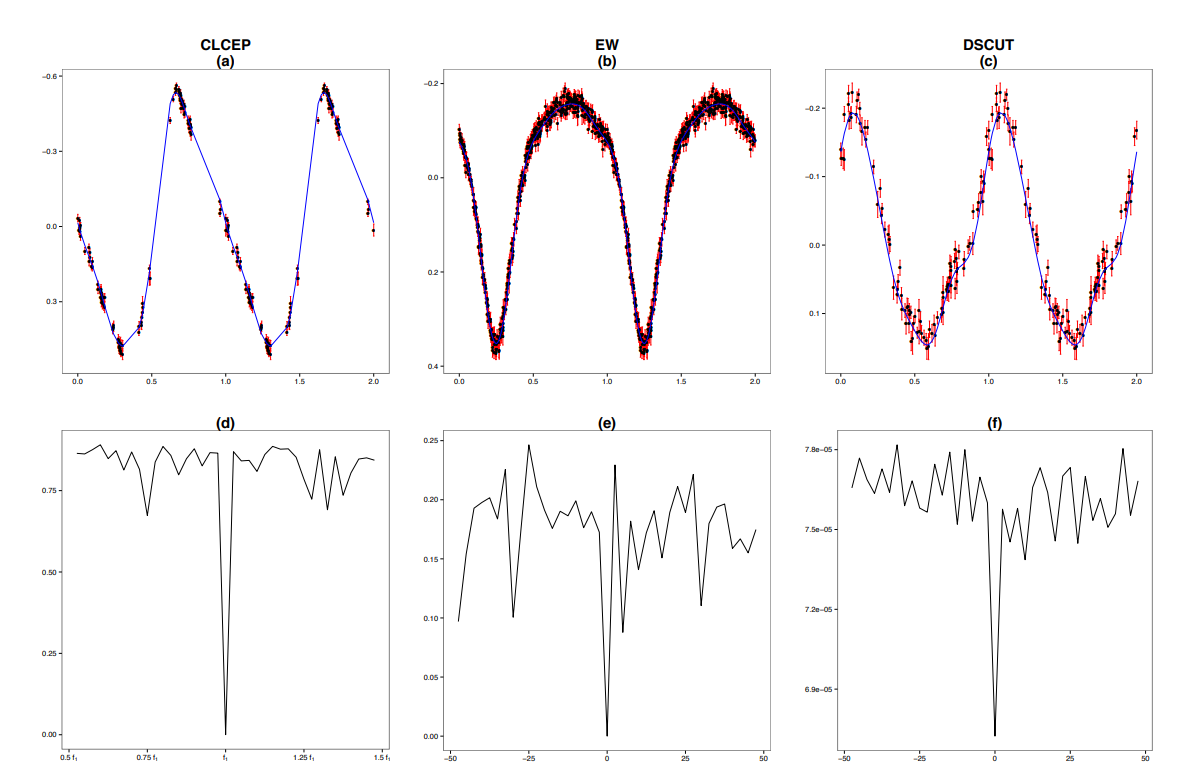
\includegraphics[scale=.2]{IAR.png}

  {\bf 1st row:} light curves of a Classical Cepheid, EW and DSCUT, respectively (harmonic best fit as continuous blue line).
  {\bf 2nd row:} Estimate of $\phi$ vs the \% of variation from the correct frequency. (Eyheramendy+2018)}
}


\frame{

  \begin{center}
    {\huge II. Fourier Analysis }
  \end{center}
}

\section{Periodic variability}

\frame{
  \frametitle{Hertzsprung--Russell diagram}
  
  \begin{center}
    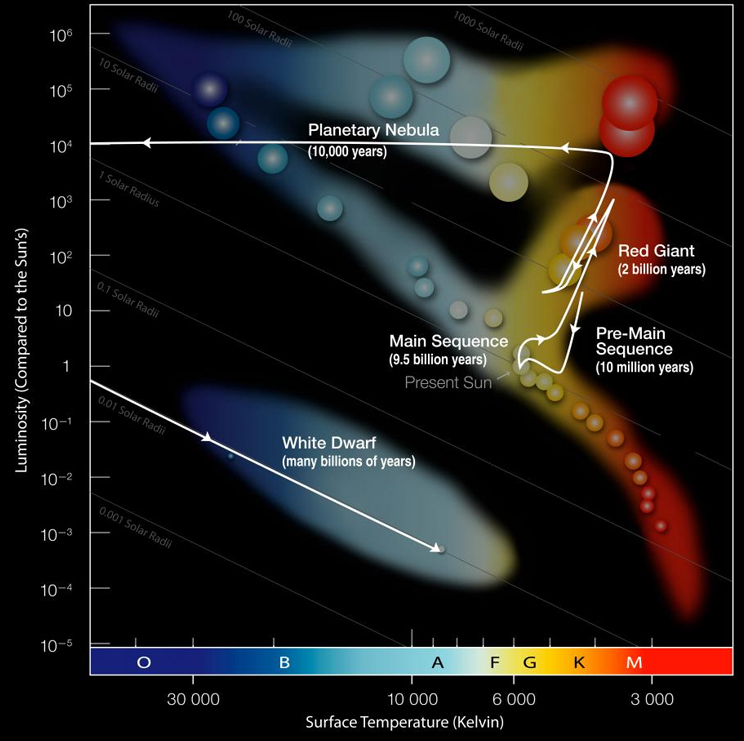
\includegraphics[scale=0.28]{evolutionary_track.jpg}
  \end{center}

  }

\frame{
  \frametitle{Hertzsprung--Russell diagram}
  
  \begin{center}
    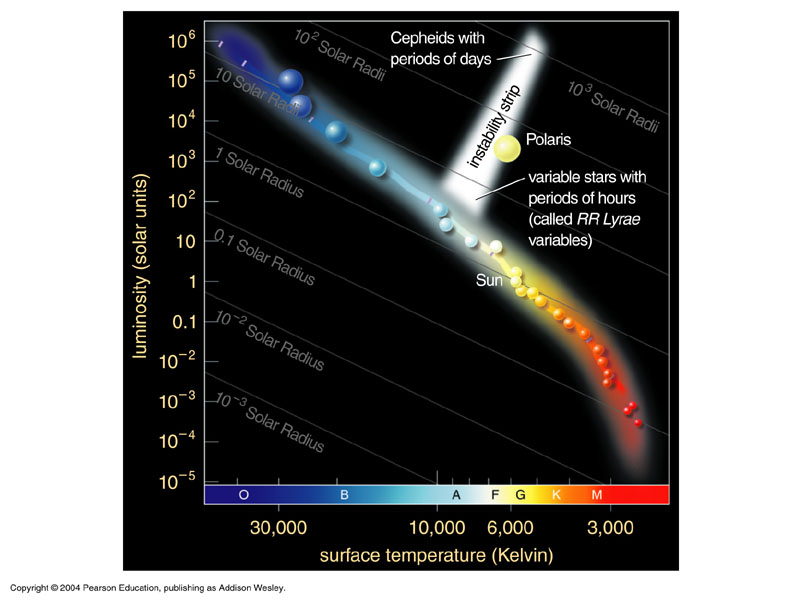
\includegraphics[scale=0.75]{HR.jpg}
  \end{center}

  }

\frame{
  \frametitle{Period--luminosity relation for some periodic stars}
  
  \begin{center}
    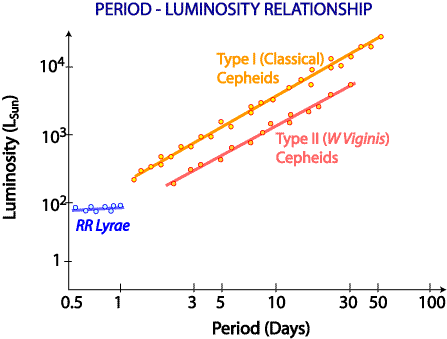
\includegraphics[scale=0.5]{periodicstars.png}
  \end{center}

  }

\frame{
  \frametitle{Period--luminosity relation for some periodic stars}
  
  \begin{center}
    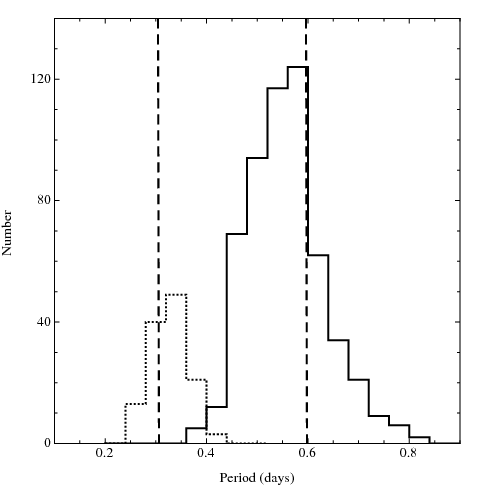
\includegraphics[scale=0.3]{Period_dist.png}
  \end{center}

  The period distributions of ab-type (solid) and c-type (dotted) RR Lyrae variables

  }



\frame{
  \frametitle{Period distribution in RR Lyrae stars}
  
  \begin{center}
    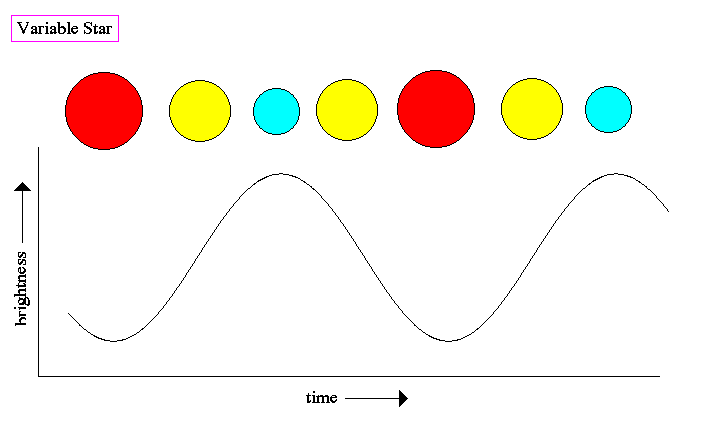
\includegraphics[scale=0.3]{variable_star.png}
  \end{center}

  The temperature and size evolution of a pulsating star in the instability strip

  }


%%%%%%%%%%%%%%%%%%%%
\section{Fourier Transform}


\frame{
  \frametitle{Fourier transform}
 
  \bi
  \item Fourier transform of $h(t)$:
  \begin{align} 
    H(f) = \int_{-\infty}^{\infty} h(t) \exp(-i~ 2 \pi ~f t) dt
    \end{align}
  \item Inverse Fourier transform of $H(f)$:
  \begin{align} 
    h(t) = \int_{-\infty}^{\infty} H(f) \exp(i~ 2 \pi ~f t) df
    \end{align}

  \ei
}

\frame{
  \frametitle{Fourier transform}
 
  \bi
\item Gaussian $N_{(0,~ \sigma)}(t)$ transform (not the same as white noise)
  \begin{align} 
    H_{Gauss}(f) &= \exp(-2 \pi^2 \sigma^2 f^2)
  \end{align}
\item Translation transform
  \begin{align}
    H_{h(t + \Delta t)}(f) &= H(f) \exp(i 2 \pi f \Delta t)
  \end{align}
\item Power spectral density
  \begin{align}
    PSD(f) &\equiv | H(f)|^2 + |H(-f)|^2,
  \end{align}
  e.g. $PSD_{\sin(2 \pi t / T)}(f) = \delta(1/T)$
%  
  \ei
}


\frame{
  \frametitle{Fourier transform}
 
  \bi
\item Parseval's theorem
  \begin{align} 
    P_{tot} &\equiv \int_{0}^{\infty} PSD(f) df = \int_{-\infty}^{\infty} |h(t)|^2 dt
  \end{align}
\item Convolution theorem
  \begin{align}
    (a \ast b)(t) &\equiv \int a(t') b(t - t') dt' \\
    H_{a \ast b}(f) &= A(f) B(f)
  \end{align}
%  
  \ei
}

\frame{
  
  \begin{center}
    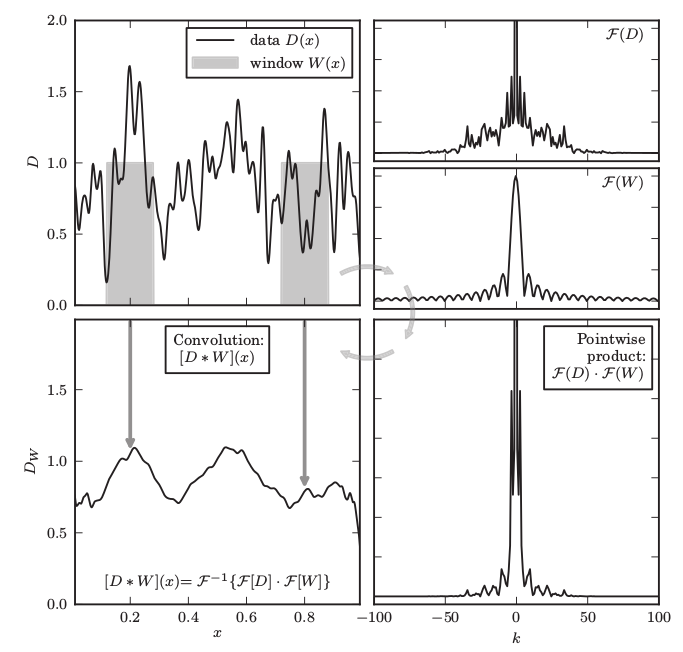
\includegraphics[scale=0.35]{convolution.png}
    
    Convolution of two function in real and Fourier space.
  \end{center}
}

\section{Discrete Fourier transform}

\frame{
  \frametitle{Discrete Fourier Transform (even sampling)}

  \bi
  \item   The discrete Fourier transform of the vector of values $h_j$ is a complex vector of length $N$ defined by:
  
    \begin{align}
      H_k = \sum_{j = 0}^{N -1} h_j \exp[-i 2 \pi j k / N],
    \end{align}
    where $k = 0, ... , (N - 1)$.

  \item   The corresponding inverse discrete Fourier transform is:
  
    \begin{align}
      h_j = \frac{1}{N} \sum_{k = 0}^{N -1} H_k \exp[i 2 \pi j k / N],
    \end{align}
    where $j = 0, ... , (N - 1)$.

    \ei
}

\frame{
  \frametitle{Nyquist sampling theorem}
  
  \bi
\item   Let us define $h(t)$ as {\bf band limited} if $H(f) = 0$ for $| f |
  > f_c$, where $f_c$ is the band limit, or the {\bf Nyquist critical
    frequency}.
\vspace{.5cm}
\item If $h(t)$ is {\bf  band  limited}:
  \bi
  \item there is some resolution limit in $t$ space, $t_c = 1 / (2 f c)$, below which $h(t)$ appears smooth.
  \item according to the {\bf Nyquist sampling theorem} we can
    \emph{exactly} reconstruct $h(t)$ from evenly sampled data when
    $\Delta t \le t_c$ as:
  \begin{align}
    h(t) = \frac{\Delta t}{t_c} \sum_{-\infty}^{\infty} h_k \frac{ \sin[ 2 \pi f_c (t - k \Delta t)]}{2 \pi f_c (t - k \Delta t)} = \frac{\Delta t}{t_c} \sum_{-\infty}^{\infty} h_k sinc[2 \pi f_c (t - k \Delta t)]
    \end{align}
\ei
\ei
  
}


\frame{
  \frametitle{Nyquist sampling theorem}
  
  \bi
  \item When the sampled function is not band limited or when the sampling rate is not sufficient (i.e. $\Delta t > t_c$) we cannot reconstruct $h(t)$

    \item In the previous case, the power spectral density from
      frequencies $| f | > f_c$ is tranferred (or {\bf aliased}) into
      the $-f_c < f < f_c$ range.

      \item The {\bf aliasing} effect can be recognized if the Fourier
        transform is nonzero at $|f| = 1 / (2 \Delta t)$.

\ei

}


\frame{

  \begin{center}

    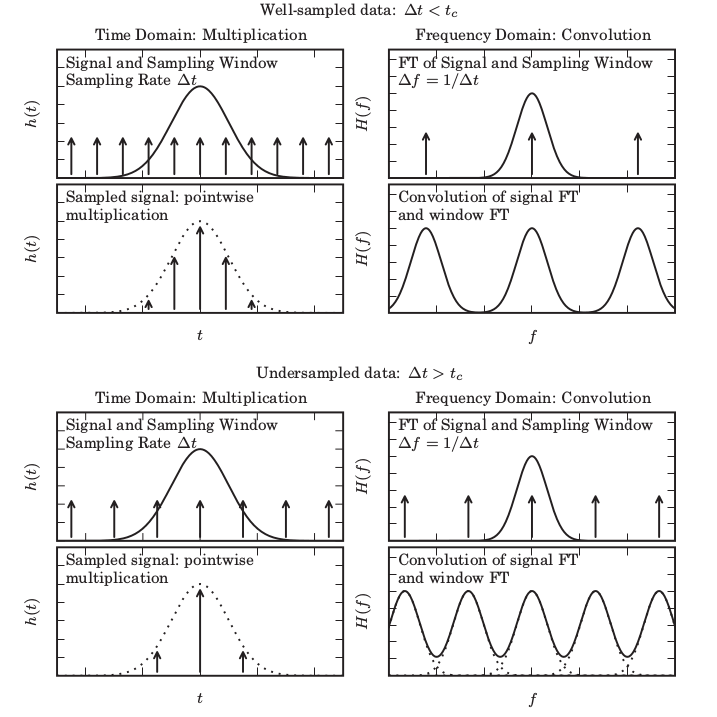
\includegraphics[scale = 0.35]{sampling.png}

    \end{center}
}


\frame{
  \frametitle{Discrete and true Fourier transform (even sampling)}

  \bi
\item The discrete Fourier transform is a good estimate of the true Fourier transform only {\bf for properly sampled and band limited functions.}
\item Then, the following relation holds:
  \begin{align}
    | H(f_k)| \approx \Delta t |H_k|,
  \end{align}
  where $f_k = k / (N \Delta t)$ for $k \le N/2$ and $f_k = (k - N) / (N \Delta t)$ for $k \ge N/2$,
\ei
}

\frame{
  \frametitle{Discrete power spectral density (even sampling)}

  \bi
\item The discrete power spectral density will be:
  \begin{align}
    PSD(f_k) = (\Delta t)^2 (|H_k|^2 + |H_{N-k}|^2).
    \end{align}
\item This can be written as:
  \begin{align}
    PSD(f_k) = 2 \biggl( \frac{T}{N} \biggr)^2 \biggl[  \biggl( \sum_{j = 0}^{N -1} h_j \cos(2 \pi f_k t_j)  \biggr)^2 + \biggl( \sum_{j = 0}^{N -1} h_j \sin(2 \pi f_k t_j)\biggr)^2  \biggr]
    \end{align}

  \ei

\begin{center}
 {\bf Note that these formulae are only valid for evenly sampled data and will be strictly valid for noiseless data.}

  \end{center}


}


\frame{
  \frametitle{Window function (even sampling)}

  \bi
  \item   The {\bf sampling window function} is the sum of delta functions placed at sampled observation times

    \item When data is evenly sampled ($\Delta t$), the Fourier
      transform of the window function is a set of evenly spaced
      deltas ($1 / \Delta t$).
      \ei
}



\frame{

  \begin{center}

    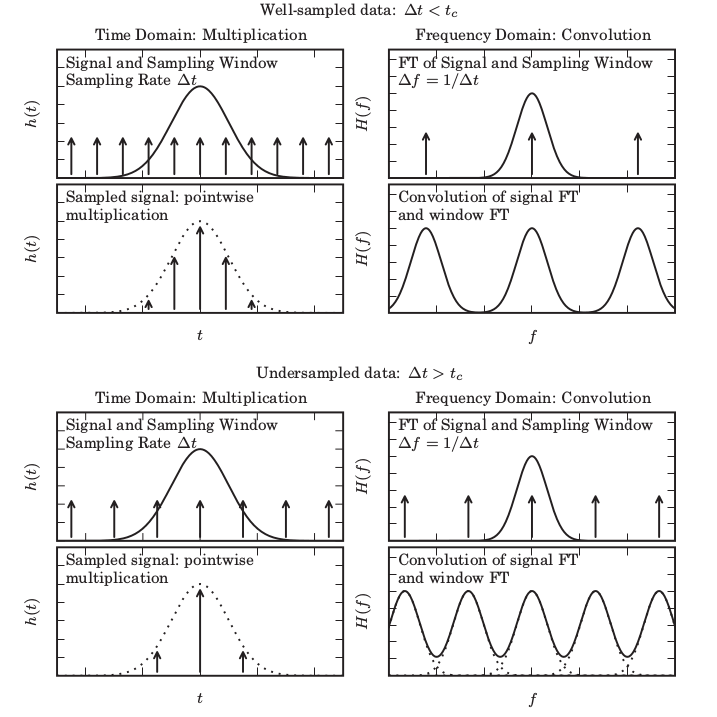
\includegraphics[scale = 0.35]{sampling.png}

    \end{center}
}

\frame{
  \frametitle{Window function (uneven sampling)}

  \bi
    \item When data is unevenly sampled, the Fourier transform of the
      window function has a more complicated structure.

    \item The power spectral density (PSD) of the window function can
      be constructed using a fine regular grid of points which are one
      near the sampling window function and zero elsewhere.

    \item The resulting PSD is called the {\bf spectral window function}

  \ei


 }

\frame{

  \begin{center}
    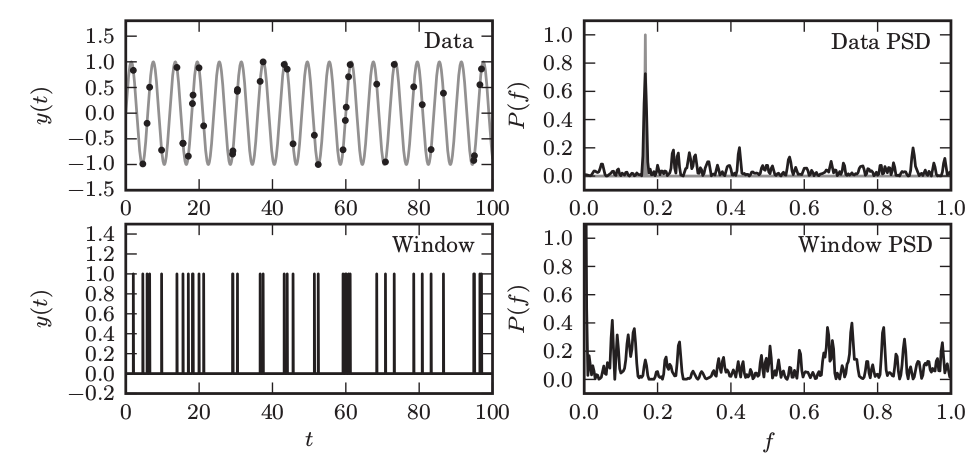
\includegraphics[scale=0.35]{windowfunction.png}

  The data is the multiplication of the true function being sampled
  with the sampling window function. The data PSD is computed from the
  convolution of the true function FT and the sampling window function
  FT.
  \end{center}

 }

\frame{
  \frametitle{Fast Fourier transform (even sampling)}

  \bi
  
\item The Fast Fourier Transform (FFT) is an algorithm for computing
  discrete Fourier transforms in $\mathcal{O}(N \log N)$ time rather
  than $\mathcal{O}$.
  
\item It is widely used for evenly sampled, high signal to noise
  ratio, timeseries data.

  \ei
 
}

\frame{

  \begin{center}
    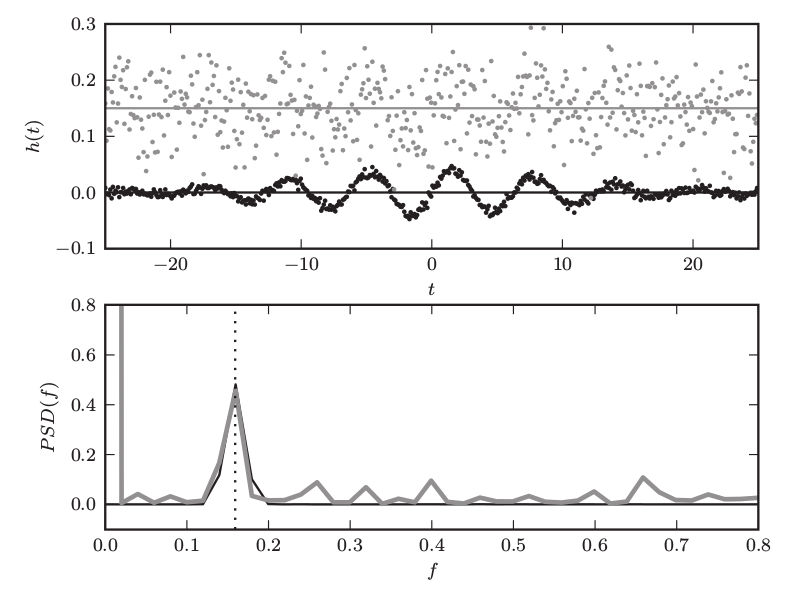
\includegraphics[scale=0.35]{FFT.png}
  \end{center}

}

%\section{Analysis of Periodic time series}


\section{Lomb--Scargle periodogram}


%\frame{
%  \frametitle{Lomb--Scargle periodogram}
%
% \bi
%
% \item The Lomb--Scargle periodogram is a standard method to search
%   for periodicity in unevenly sampled timeseries data. It is defined as:
%
%   \begin{align}
%     P_{LS}(\omega) &= \frac{1}{2} \biggl[ \frac{R^2(\omega)}{C(\omega)} + \frac{I^2(\omega)}{S(\omega)} \biggr],
%   \end{align}
%   where
%   \tiny{
%   \begin{al0ign}
%     V &= \sum_{j=1}^{N} \omega_j (y_j - \bar y)^2, ~~~~\bar y = \sum \omega_j y_j, ~~~~ \omega_j = \frac{1}{W} \frac{1}{\sigma_j^2}, ~~~~ W = \sum_{j=1}^N \frac{1}{\sigma_j^2} \\
%     R(\omega) &= \sum_{j=1}^N \omega_j (y_j - \bar y) \cos[\omega (t_j - \tau)], ~~~~ I(\omega) = \sum_{j=1}^N \omega_j (y_j - \bar y) \sin[\omega (t_j - \tau)] \\
%     C(\omega) &= \sum_{j=1}^N \omega_j (y_j - \bar y) \cos^2[\omega (t_j - \tau)], ~~~~ I(\omega) = \sum_{j=1}^N \omega_j (y_j - \bar y) \sin^2[\omega (t_j - \tau)] \\
%     \tan(2 \omega \tau) &= \frac{\sum_{j=1}^N \omega_j \sin(2 \omega t_j)}{\sum_{j=1}^N \omega_j \cos(2 \omega t_j)}
%     \end{align}
%}
%   
%   \ei
%   
%}


\frame{
  \frametitle{Lomb--Scargle periodogram}

 \bi

 \item The Lomb--Scargle periodogram is a standard method to search
   for periodicity in unevenly sampled timeseries data. It is defined as:

   \begin{align}
     P_{LS}(\omega) &= \frac{1}{2} \biggl[ \frac{\biggl(\sum_{j=1}^N X_j \cos[\omega (t_j - \tau)]\biggr)^2}{\sum_{j=1}^N \cos^2[\omega (t_j - \tau)]} + \frac{\biggl( \sum_{j=1}^N X_j \sin[\omega (t_j - \tau)] \biggr)^2}{\sum_{j=1}^N \sin^2[\omega (t_j - \tau)]} \biggr],
   \end{align}
   where $\tau$ is defined by
   \begin{align}
     \tan(2 \omega \tau) &= \frac{\sum_{j=1}^N \sin(2 \omega t_j)}{\sum_{j=1}^N \cos(2 \omega t_j)}
     \end{align}
   
   \ei
   
}

\frame{
  \frametitle{Lomb--Scargle periodogram}
  
  \bi
  \item The Lomb--Scargle periodogram has two main advantages:
    \bi
    \item It has a simple statistical behaviour by design, allowing a
      simple evaluation of the statistical significance of its peaks
      \item It is equivalent to the reduction of the sum of squares in
        least--squares fitting of sine waves to the data.
 \ei

\ei

}

\frame{
  \frametitle{Lomb--Scargle periodrogram: statistical significance}
  
  \bi
  \item $P_{LS}(\omega)$ is a random variable.

  \item We must answer the question: \emph{What is the probability that a feature is due to random statistical fluctuations?}

    \item If $Z \equiv P_{LS}(\omega)$ one can show

      \begin{align}
        p_{Z}(z)  dz &= Pr(z < Z < z + dz) = \exp(-z) dz\\
        Pr(Z<z) &= \int_0^z  p_{Z}(z') dz' = 1 - \exp(-z)\\
        Pr(Z > z) &= \exp(-z),
      \end{align}
      which is the probability of a large observed power at a given
      frequency.

 \ei
}

\frame{
  \frametitle{Lomb--Scargle periodrogram: statistical significance}
  
  \bi
    \item For many peaks one has to apply a penalty for inspecting many values:
      \begin{align}
        Pr(Z > z)\biggl|_{P_{LS}^{\max}(\omega)} = 1 - (1 - \exp(-z))^N
      \end{align}

  \item In fact, the expected maximum of a pure noise spectrum over a set of $N$ frequencies is:
    \begin{align}
      <Z_{\max}> = \sum_{k =1}^N \frac{1}{k},
    \end{align}
    which diverges logarithmically with N.
    
    \item The previous point means that if enough frequencies are
      inspected, a significant peak will eventually be found if no
      penalty is applied.
    

    \ei

}

\frame{
  \frametitle{Lomb--Scargle periodrogram: statistical significance}

  \bi
  
  \item The periodogram threshold $z_0$ such that a detection is spurious only with a small probability $p_0$ is:

    
    $z_0 = -\ln \bigg(1 - (1 - p_0)^{1 / N}\biggr)$

    \item Given the threshold $z_0$, the probability of missing a signal of power P is given by:

      $P_{miss} = (1 - p_0)^{1 - 1/N} \biggl\lbrace \lbrace 1 - \exp [-(z_0 + P)] \rbrace \phi(z_0, P) \biggr\rbrace$,

      where $\phi(x, y) = \sum_{m = 0}^\infty \sum_{k = 0}^\infty x^k  y^m / (k! m!)$

    \ei
    

}

\frame{

  \begin{center}

    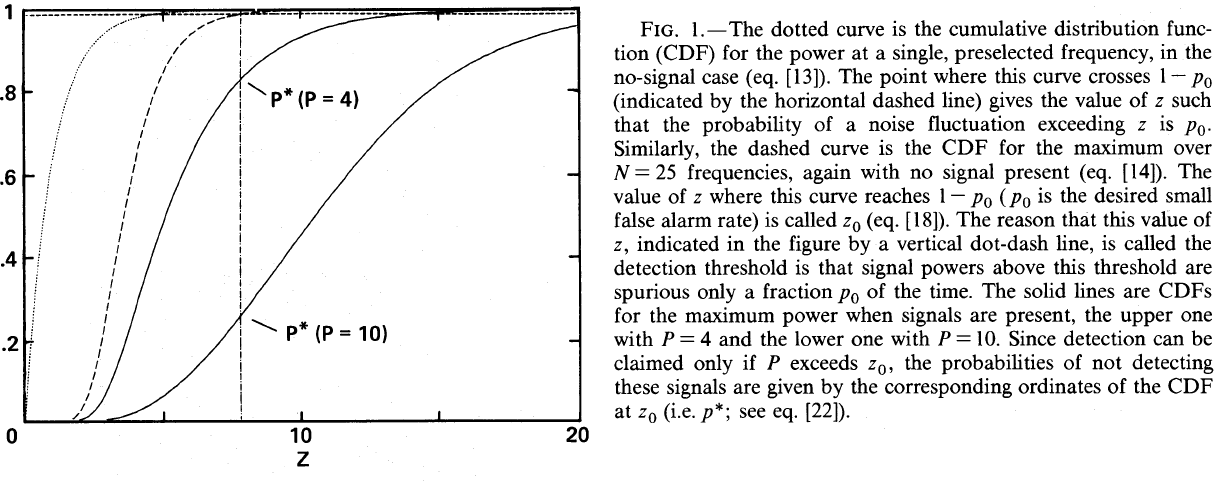
\includegraphics[scale = 0.27]{Scargle.png}

    Scargle 1982, ApJ

    \end{center}
}

\frame{
  \frametitle{Lomb--Scargle periodrogram: practical application}

  \bi
  \item Given that we must choose carefully which frequency peaks to explore, it is important to understand what frequency range will be meaninful

    \item For the minimum frequency we can choose $\omega_{\min} = 2 \pi / (T_{\max} - T_{\min})$

    \item When the sampling is even, the maximum frequency that can be explored is $\omega_{\max} = 2 \pi / \Delta t$.

    \item For the frequency steps, we can choose $\Delta \omega = \eta \omega_{\min}$, with $\eta = 0.1$

\ei
}


\frame{
  \frametitle{Lomb--Scargle periodrogram: practical application}

  \bi

    \item When the sampling is uneven, the maximum frequency to
      explore is not obvious. 

\item e.g. the median value of $2 \pi / \Delta t_i$ can be a gross
  underestimate because sometimes uneven sampling can detect
  periodicity with frequencies even higher than $2 \pi / \Delta
  t_{\min}$ (Eyer \& Bartoldi 1999)

  \item a very conservative hard limit is to use $2 \pi / T_{exp}$,
    where $T_{exp}$ is the exposure time, but in practice one must
    look at the phase coverage of the maximum frequency chosen.

      \item See \href{https://arxiv.org/pdf/1703.09824.pdf}{``Understanding the Lomb-Scargle Periodogram''} by Jake VanderPlas

  \ei

}

\frame{

  \begin{center}

    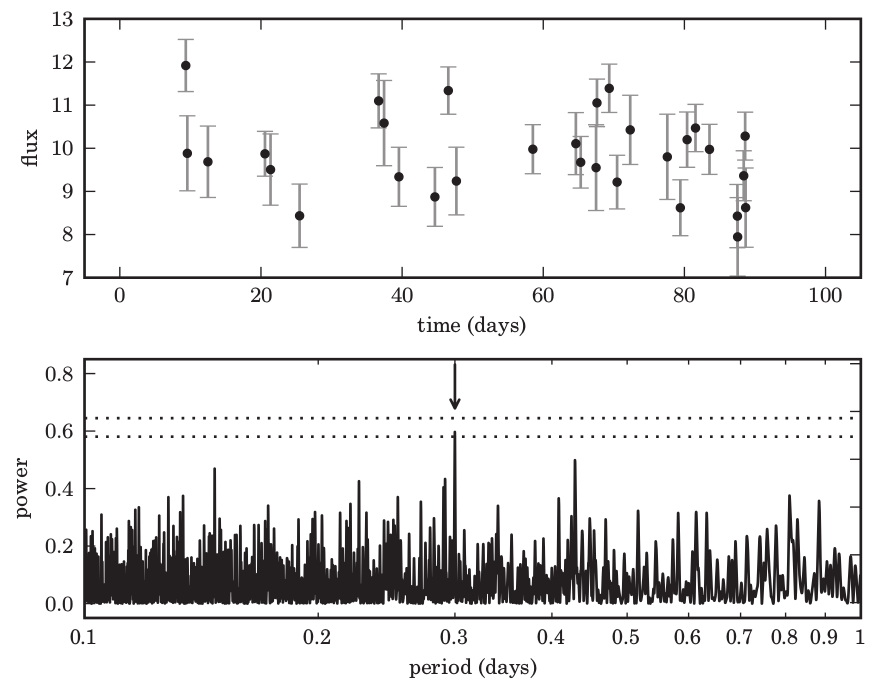
\includegraphics[scale = 0.27]{LS.png}

    Lomb--Scargle periodogram for $y(t) = 10 + \sin( 2 \pi t / P)$,
    with $P = 0.3$ and heteroscedastic errors with a uniform
    distribution for the standard deviations between 0.5 and 1.
    
    \end{center}
}


\frame{
  \frametitle{Generalized Lomb--Scargle periodrogram}

  \bi
  \item A generalization of the Lomb--Scargle method (Zechmeister \&
    K\"urster 2009, A\& A) includes an offset term to the model

    \item This results in much better detection efficiencies when the
      mean of the distribution is overestimated due to an unlucky
      choice of the sampling window function.

      \item Both the Lomb--Scargle and generalized Lomb--Scargle
        methods are implemented in Python library AstroML (lomb\_scargle)

\ei
}

\frame{

  \begin{center}

    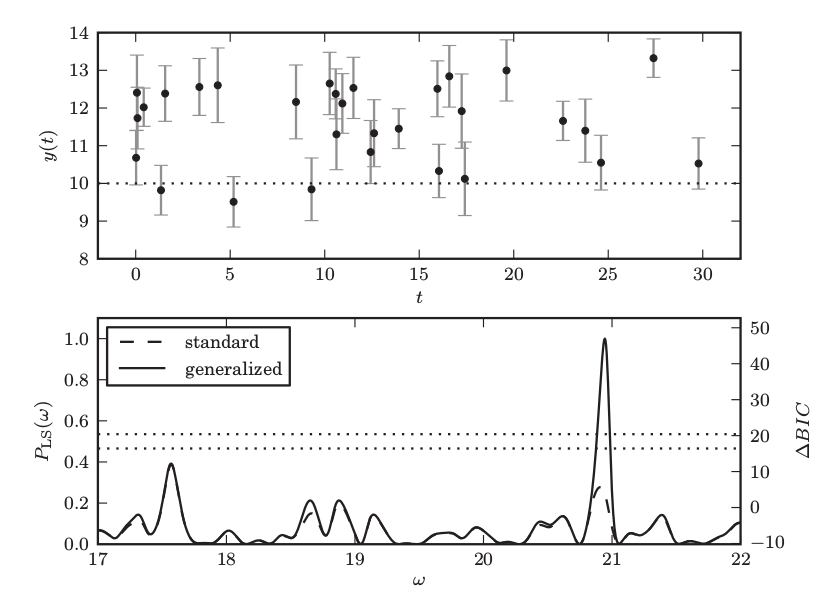
\includegraphics[scale = 0.27]{LSvsGLS.png}

    Lomb--Scargle vs generalized Lomb--Scargle periodogram for $y(t) =
    10 + \sin( 2 \pi t / P)$, with $P = 0.3$ and heteroscedastic
    errors with a uniform distribution for the standard deviations
    between 0.5 and 1. The sampling window function was chosen to
    overestimate the true mean.
    
    \end{center}
}

\frame{

  \begin{center}

    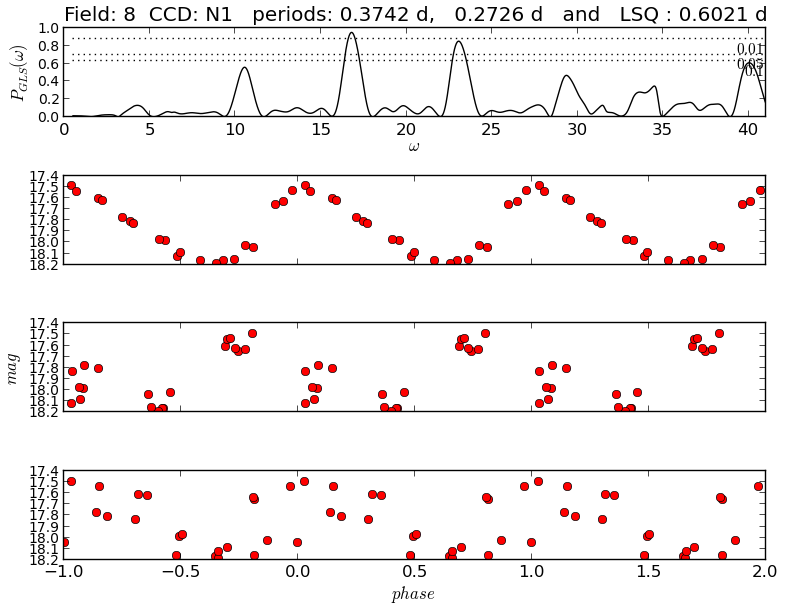
\includegraphics[scale = 0.36]{GMedina.png}

    Candidate RR Lyrae star obtained with DECam (credit: G. Medina)
    \end{center}
}

\frame{

  \begin{center}

    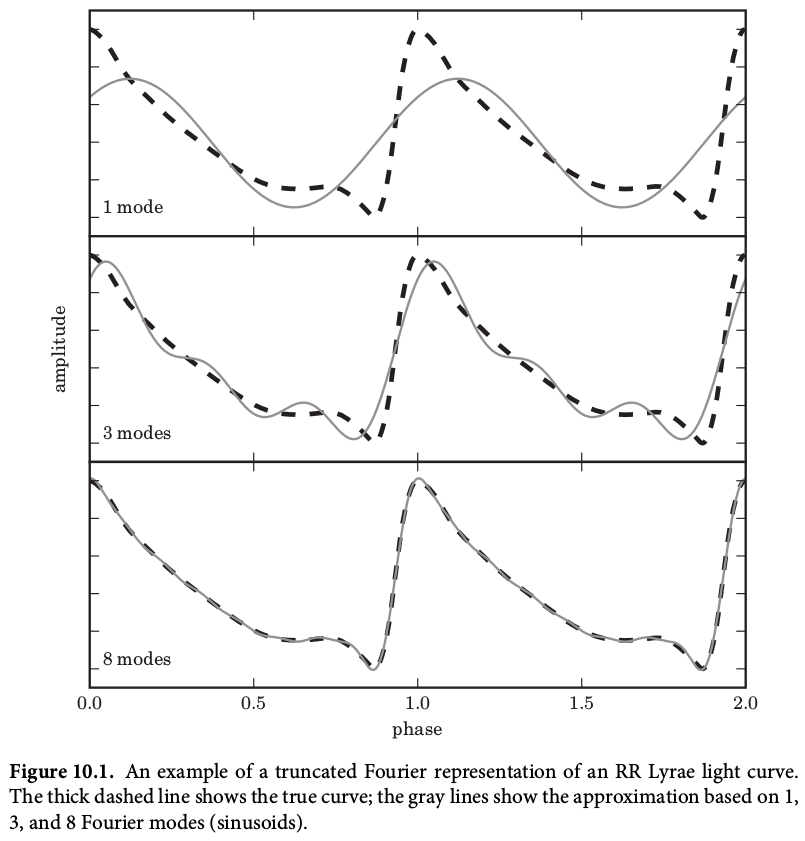
\includegraphics[scale = 0.27]{RRLyrae.png}

    \end{center}
}


\section{Other methods}

\frame{
  \frametitle{Other methods}

  \bi
\item When the underlying variability has a complex spectral
  structure one needs to use other methods, e.g.:
  
  \bi
\item Truncated Fourier Series Model (implemented in AstroML as multiterm\_periodogram)
  
\item Correntropy methods (Huijse, P. et al. 2011, 2012, IEEE Transactions)
  
  \ei
  
  \ei
  
}


\section{Summary}

\frame{
  \frametitle{Summary}

  \bi
  
  \item Astronomical timeseries are unevenly sampled, have heteroscedastic errors and low signal to noise

  \item Some important concepts: autocovariance and autocorrelation,
    $1/f^\gamma$ noise, power spectral density, sampling and spectral
    window function, periodogram, Lomb--Scargle periodogram

  \item For non--periodic autocorrelated variability use
    autoregressive modelling like ARMA and its derivatives.

  \item For periodic signals, work in the frequency domain and use the
    generalized Lomb-Scargle method.  When the underlying light curve
    cannot be represented by a few Fourier terms use more
    sophisticated methods.

  \ei

}



%\frame {
%	\frametitle{Periodogram}
%	This text will stay on all pages.
%	\only<1>{
%		\begin{itemize}
%			\item<1->This will only appear on the first page
%			\item<1->This is also only for the first page
%		\end{itemize}
%	}
%	\only<2>{
%		\begin{itemize}
%			\item<2->This will only appear on the second page
%		\item<2->This is also only for the second page
%		\end{itemize}
%      }
%}

%\subsection{Second Sub Section}
%
%\frame {
%	\frametitle{Last Frame}
%	This is the last frame
%}

\end{document}
